% Options for packages loaded elsewhere
\PassOptionsToPackage{unicode}{hyperref}
\PassOptionsToPackage{hyphens}{url}
\PassOptionsToPackage{dvipsnames,svgnames,x11names}{xcolor}
%
\documentclass[
  letterpaper,
  DIV=11,
  numbers=noendperiod]{scrartcl}

\usepackage{amsmath,amssymb}
\usepackage{iftex}
\ifPDFTeX
  \usepackage[T1]{fontenc}
  \usepackage[utf8]{inputenc}
  \usepackage{textcomp} % provide euro and other symbols
\else % if luatex or xetex
  \usepackage{unicode-math}
  \defaultfontfeatures{Scale=MatchLowercase}
  \defaultfontfeatures[\rmfamily]{Ligatures=TeX,Scale=1}
\fi
\usepackage{lmodern}
\ifPDFTeX\else  
    % xetex/luatex font selection
\fi
% Use upquote if available, for straight quotes in verbatim environments
\IfFileExists{upquote.sty}{\usepackage{upquote}}{}
\IfFileExists{microtype.sty}{% use microtype if available
  \usepackage[]{microtype}
  \UseMicrotypeSet[protrusion]{basicmath} % disable protrusion for tt fonts
}{}
\makeatletter
\@ifundefined{KOMAClassName}{% if non-KOMA class
  \IfFileExists{parskip.sty}{%
    \usepackage{parskip}
  }{% else
    \setlength{\parindent}{0pt}
    \setlength{\parskip}{6pt plus 2pt minus 1pt}}
}{% if KOMA class
  \KOMAoptions{parskip=half}}
\makeatother
\usepackage{xcolor}
\setlength{\emergencystretch}{3em} % prevent overfull lines
\setcounter{secnumdepth}{-\maxdimen} % remove section numbering
% Make \paragraph and \subparagraph free-standing
\ifx\paragraph\undefined\else
  \let\oldparagraph\paragraph
  \renewcommand{\paragraph}[1]{\oldparagraph{#1}\mbox{}}
\fi
\ifx\subparagraph\undefined\else
  \let\oldsubparagraph\subparagraph
  \renewcommand{\subparagraph}[1]{\oldsubparagraph{#1}\mbox{}}
\fi

\usepackage{color}
\usepackage{fancyvrb}
\newcommand{\VerbBar}{|}
\newcommand{\VERB}{\Verb[commandchars=\\\{\}]}
\DefineVerbatimEnvironment{Highlighting}{Verbatim}{commandchars=\\\{\}}
% Add ',fontsize=\small' for more characters per line
\usepackage{framed}
\definecolor{shadecolor}{RGB}{241,243,245}
\newenvironment{Shaded}{\begin{snugshade}}{\end{snugshade}}
\newcommand{\AlertTok}[1]{\textcolor[rgb]{0.68,0.00,0.00}{#1}}
\newcommand{\AnnotationTok}[1]{\textcolor[rgb]{0.37,0.37,0.37}{#1}}
\newcommand{\AttributeTok}[1]{\textcolor[rgb]{0.40,0.45,0.13}{#1}}
\newcommand{\BaseNTok}[1]{\textcolor[rgb]{0.68,0.00,0.00}{#1}}
\newcommand{\BuiltInTok}[1]{\textcolor[rgb]{0.00,0.23,0.31}{#1}}
\newcommand{\CharTok}[1]{\textcolor[rgb]{0.13,0.47,0.30}{#1}}
\newcommand{\CommentTok}[1]{\textcolor[rgb]{0.37,0.37,0.37}{#1}}
\newcommand{\CommentVarTok}[1]{\textcolor[rgb]{0.37,0.37,0.37}{\textit{#1}}}
\newcommand{\ConstantTok}[1]{\textcolor[rgb]{0.56,0.35,0.01}{#1}}
\newcommand{\ControlFlowTok}[1]{\textcolor[rgb]{0.00,0.23,0.31}{#1}}
\newcommand{\DataTypeTok}[1]{\textcolor[rgb]{0.68,0.00,0.00}{#1}}
\newcommand{\DecValTok}[1]{\textcolor[rgb]{0.68,0.00,0.00}{#1}}
\newcommand{\DocumentationTok}[1]{\textcolor[rgb]{0.37,0.37,0.37}{\textit{#1}}}
\newcommand{\ErrorTok}[1]{\textcolor[rgb]{0.68,0.00,0.00}{#1}}
\newcommand{\ExtensionTok}[1]{\textcolor[rgb]{0.00,0.23,0.31}{#1}}
\newcommand{\FloatTok}[1]{\textcolor[rgb]{0.68,0.00,0.00}{#1}}
\newcommand{\FunctionTok}[1]{\textcolor[rgb]{0.28,0.35,0.67}{#1}}
\newcommand{\ImportTok}[1]{\textcolor[rgb]{0.00,0.46,0.62}{#1}}
\newcommand{\InformationTok}[1]{\textcolor[rgb]{0.37,0.37,0.37}{#1}}
\newcommand{\KeywordTok}[1]{\textcolor[rgb]{0.00,0.23,0.31}{#1}}
\newcommand{\NormalTok}[1]{\textcolor[rgb]{0.00,0.23,0.31}{#1}}
\newcommand{\OperatorTok}[1]{\textcolor[rgb]{0.37,0.37,0.37}{#1}}
\newcommand{\OtherTok}[1]{\textcolor[rgb]{0.00,0.23,0.31}{#1}}
\newcommand{\PreprocessorTok}[1]{\textcolor[rgb]{0.68,0.00,0.00}{#1}}
\newcommand{\RegionMarkerTok}[1]{\textcolor[rgb]{0.00,0.23,0.31}{#1}}
\newcommand{\SpecialCharTok}[1]{\textcolor[rgb]{0.37,0.37,0.37}{#1}}
\newcommand{\SpecialStringTok}[1]{\textcolor[rgb]{0.13,0.47,0.30}{#1}}
\newcommand{\StringTok}[1]{\textcolor[rgb]{0.13,0.47,0.30}{#1}}
\newcommand{\VariableTok}[1]{\textcolor[rgb]{0.07,0.07,0.07}{#1}}
\newcommand{\VerbatimStringTok}[1]{\textcolor[rgb]{0.13,0.47,0.30}{#1}}
\newcommand{\WarningTok}[1]{\textcolor[rgb]{0.37,0.37,0.37}{\textit{#1}}}

\providecommand{\tightlist}{%
  \setlength{\itemsep}{0pt}\setlength{\parskip}{0pt}}\usepackage{longtable,booktabs,array}
\usepackage{calc} % for calculating minipage widths
% Correct order of tables after \paragraph or \subparagraph
\usepackage{etoolbox}
\makeatletter
\patchcmd\longtable{\par}{\if@noskipsec\mbox{}\fi\par}{}{}
\makeatother
% Allow footnotes in longtable head/foot
\IfFileExists{footnotehyper.sty}{\usepackage{footnotehyper}}{\usepackage{footnote}}
\makesavenoteenv{longtable}
\usepackage{graphicx}
\makeatletter
\def\maxwidth{\ifdim\Gin@nat@width>\linewidth\linewidth\else\Gin@nat@width\fi}
\def\maxheight{\ifdim\Gin@nat@height>\textheight\textheight\else\Gin@nat@height\fi}
\makeatother
% Scale images if necessary, so that they will not overflow the page
% margins by default, and it is still possible to overwrite the defaults
% using explicit options in \includegraphics[width, height, ...]{}
\setkeys{Gin}{width=\maxwidth,height=\maxheight,keepaspectratio}
% Set default figure placement to htbp
\makeatletter
\def\fps@figure{htbp}
\makeatother

\usepackage{pdflscape}
\KOMAoption{captions}{tableheading}
\makeatletter
\@ifpackageloaded{tcolorbox}{}{\usepackage[skins,breakable]{tcolorbox}}
\@ifpackageloaded{fontawesome5}{}{\usepackage{fontawesome5}}
\definecolor{quarto-callout-color}{HTML}{909090}
\definecolor{quarto-callout-note-color}{HTML}{0758E5}
\definecolor{quarto-callout-important-color}{HTML}{CC1914}
\definecolor{quarto-callout-warning-color}{HTML}{EB9113}
\definecolor{quarto-callout-tip-color}{HTML}{00A047}
\definecolor{quarto-callout-caution-color}{HTML}{FC5300}
\definecolor{quarto-callout-color-frame}{HTML}{acacac}
\definecolor{quarto-callout-note-color-frame}{HTML}{4582ec}
\definecolor{quarto-callout-important-color-frame}{HTML}{d9534f}
\definecolor{quarto-callout-warning-color-frame}{HTML}{f0ad4e}
\definecolor{quarto-callout-tip-color-frame}{HTML}{02b875}
\definecolor{quarto-callout-caution-color-frame}{HTML}{fd7e14}
\makeatother
\makeatletter
\@ifpackageloaded{caption}{}{\usepackage{caption}}
\AtBeginDocument{%
\ifdefined\contentsname
  \renewcommand*\contentsname{Table of contents}
\else
  \newcommand\contentsname{Table of contents}
\fi
\ifdefined\listfigurename
  \renewcommand*\listfigurename{List of Figures}
\else
  \newcommand\listfigurename{List of Figures}
\fi
\ifdefined\listtablename
  \renewcommand*\listtablename{List of Tables}
\else
  \newcommand\listtablename{List of Tables}
\fi
\ifdefined\figurename
  \renewcommand*\figurename{Figure}
\else
  \newcommand\figurename{Figure}
\fi
\ifdefined\tablename
  \renewcommand*\tablename{Table}
\else
  \newcommand\tablename{Table}
\fi
}
\@ifpackageloaded{float}{}{\usepackage{float}}
\floatstyle{ruled}
\@ifundefined{c@chapter}{\newfloat{codelisting}{h}{lop}}{\newfloat{codelisting}{h}{lop}[chapter]}
\floatname{codelisting}{Listing}
\newcommand*\listoflistings{\listof{codelisting}{List of Listings}}
\makeatother
\makeatletter
\makeatother
\makeatletter
\@ifpackageloaded{caption}{}{\usepackage{caption}}
\@ifpackageloaded{subcaption}{}{\usepackage{subcaption}}
\makeatother
\ifLuaTeX
  \usepackage{selnolig}  % disable illegal ligatures
\fi
\usepackage{bookmark}

\IfFileExists{xurl.sty}{\usepackage{xurl}}{} % add URL line breaks if available
\urlstyle{same} % disable monospaced font for URLs
\hypersetup{
  colorlinks=true,
  linkcolor={blue},
  filecolor={Maroon},
  citecolor={Blue},
  urlcolor={Blue},
  pdfcreator={LaTeX via pandoc}}

\author{}
\date{}

\begin{document}

\section{Funciones y Clases}\label{sec-funciones_clases}

\subsection{Funciones j\_eval y j\_plot en
R}\label{funciones-j_eval-y-j_plot-en-r}

\begin{Shaded}
\begin{Highlighting}[]
\CommentTok{\# \#| include: false}
\FunctionTok{source}\NormalTok{(}\StringTok{"./docs/j\_eval\_j\_plot.r"}\NormalTok{)}
\end{Highlighting}
\end{Shaded}

\subsection{Introducción}\label{introducciuxf3n}

Hasta ahora, hemos escrito código que se ejecuta de arriba hacia abajo,
como una lista de mercado. Pero en proyectos reales de geomática,
necesitamos reutilizar lógica. Si tienes un cálculo complejo para medir
distancias o para valuar un predio, no quieres copiar y pegar ese código
cien veces.

Para eso existen las \textbf{funciones} (máquinas que procesan datos) y
las \textbf{clases} (moldes para crear objetos complejos). En este
capítulo aprenderás a encapsular tu lógica para que tu código sea
modular, limpio y fácil de mantener.

\subsection{Objetivos de aprendizaje}\label{objetivos-de-aprendizaje}

\begin{itemize}
\tightlist
\item
  Crear funciones reutilizables para automatizar cálculos espaciales
  recurrentes.
\item
  Manejar parámetros opcionales, valores por defecto y argumentos
  dinámicos.
\item
  Entender los principios básicos de la Programación Orientada a Objetos
  (POO) para modelar elementos del mundo real.
\end{itemize}

\subsection{1. Funciones: bloques de código
reutilizables}\label{funciones-bloques-de-cuxf3digo-reutilizables}

Una función es como una receta de cocina: tú le pasas los ingredientes
(parámetros de entrada), ella realiza un proceso interno (cuerpo de la
función) y te entrega un resultado (valor de retorno).

Para ilustrar el poder de las funciones, vamos a construir tres
herramientas fundamentales para cualquier analista espacial. Cada una
nos enseñará un concepto nuevo de programación:

\begin{enumerate}
\def\labelenumi{\arabic{enumi}.}
\tightlist
\item
  \textbf{La calculadora matemática (\texttt{haversine}):} Resolveremos
  el cálculo de la distancia entre dos ciudades. Como la Tierra no es
  plana, no podemos usar una simple línea recta (Pitágoras).
\item
  \textbf{El procesador por lotes (\texttt{medir\_ruta}):} Crearemos una
  función que reciba una lista completa de coordenadas, la recorra con
  un ciclo \texttt{for} y llame a nuestra primera función
  (\texttt{haversine}) repetidas veces para medir los tramos de una
  ruta.
\item
  \textbf{El recolector dinámico (\texttt{describir\_punto}):} Crearemos
  una función que use \textbf{argumentos dinámicos} (\texttt{**kwargs}
  en Python, \texttt{...} en R y \texttt{kwargs...} en Julia) para
  atrapar cualquier cantidad de variables extra (clima, población, etc.)
  que el usuario decida enviarnos.
\end{enumerate}

\subsubsection{La matemática detrás de nuestra calculadora
espacial}\label{la-matemuxe1tica-detruxe1s-de-nuestra-calculadora-espacial}

La \textbf{fórmula de Haversine} calcula la distancia de círculo máximo
(\emph{great-circle distance}) (Figure~\ref{fig-great_circle}) entre dos
puntos en la superficie de una esfera, como la Tierra, a partir de sus
coordenadas de latitud y longitud. La fórmula tiene en cuenta la
curvatura de la esfera, lo que la hace mucho más precisa que una simple
distancia euclidiana (línea recta) para aplicaciones geoespaciales.

\begin{figure}

\centering{

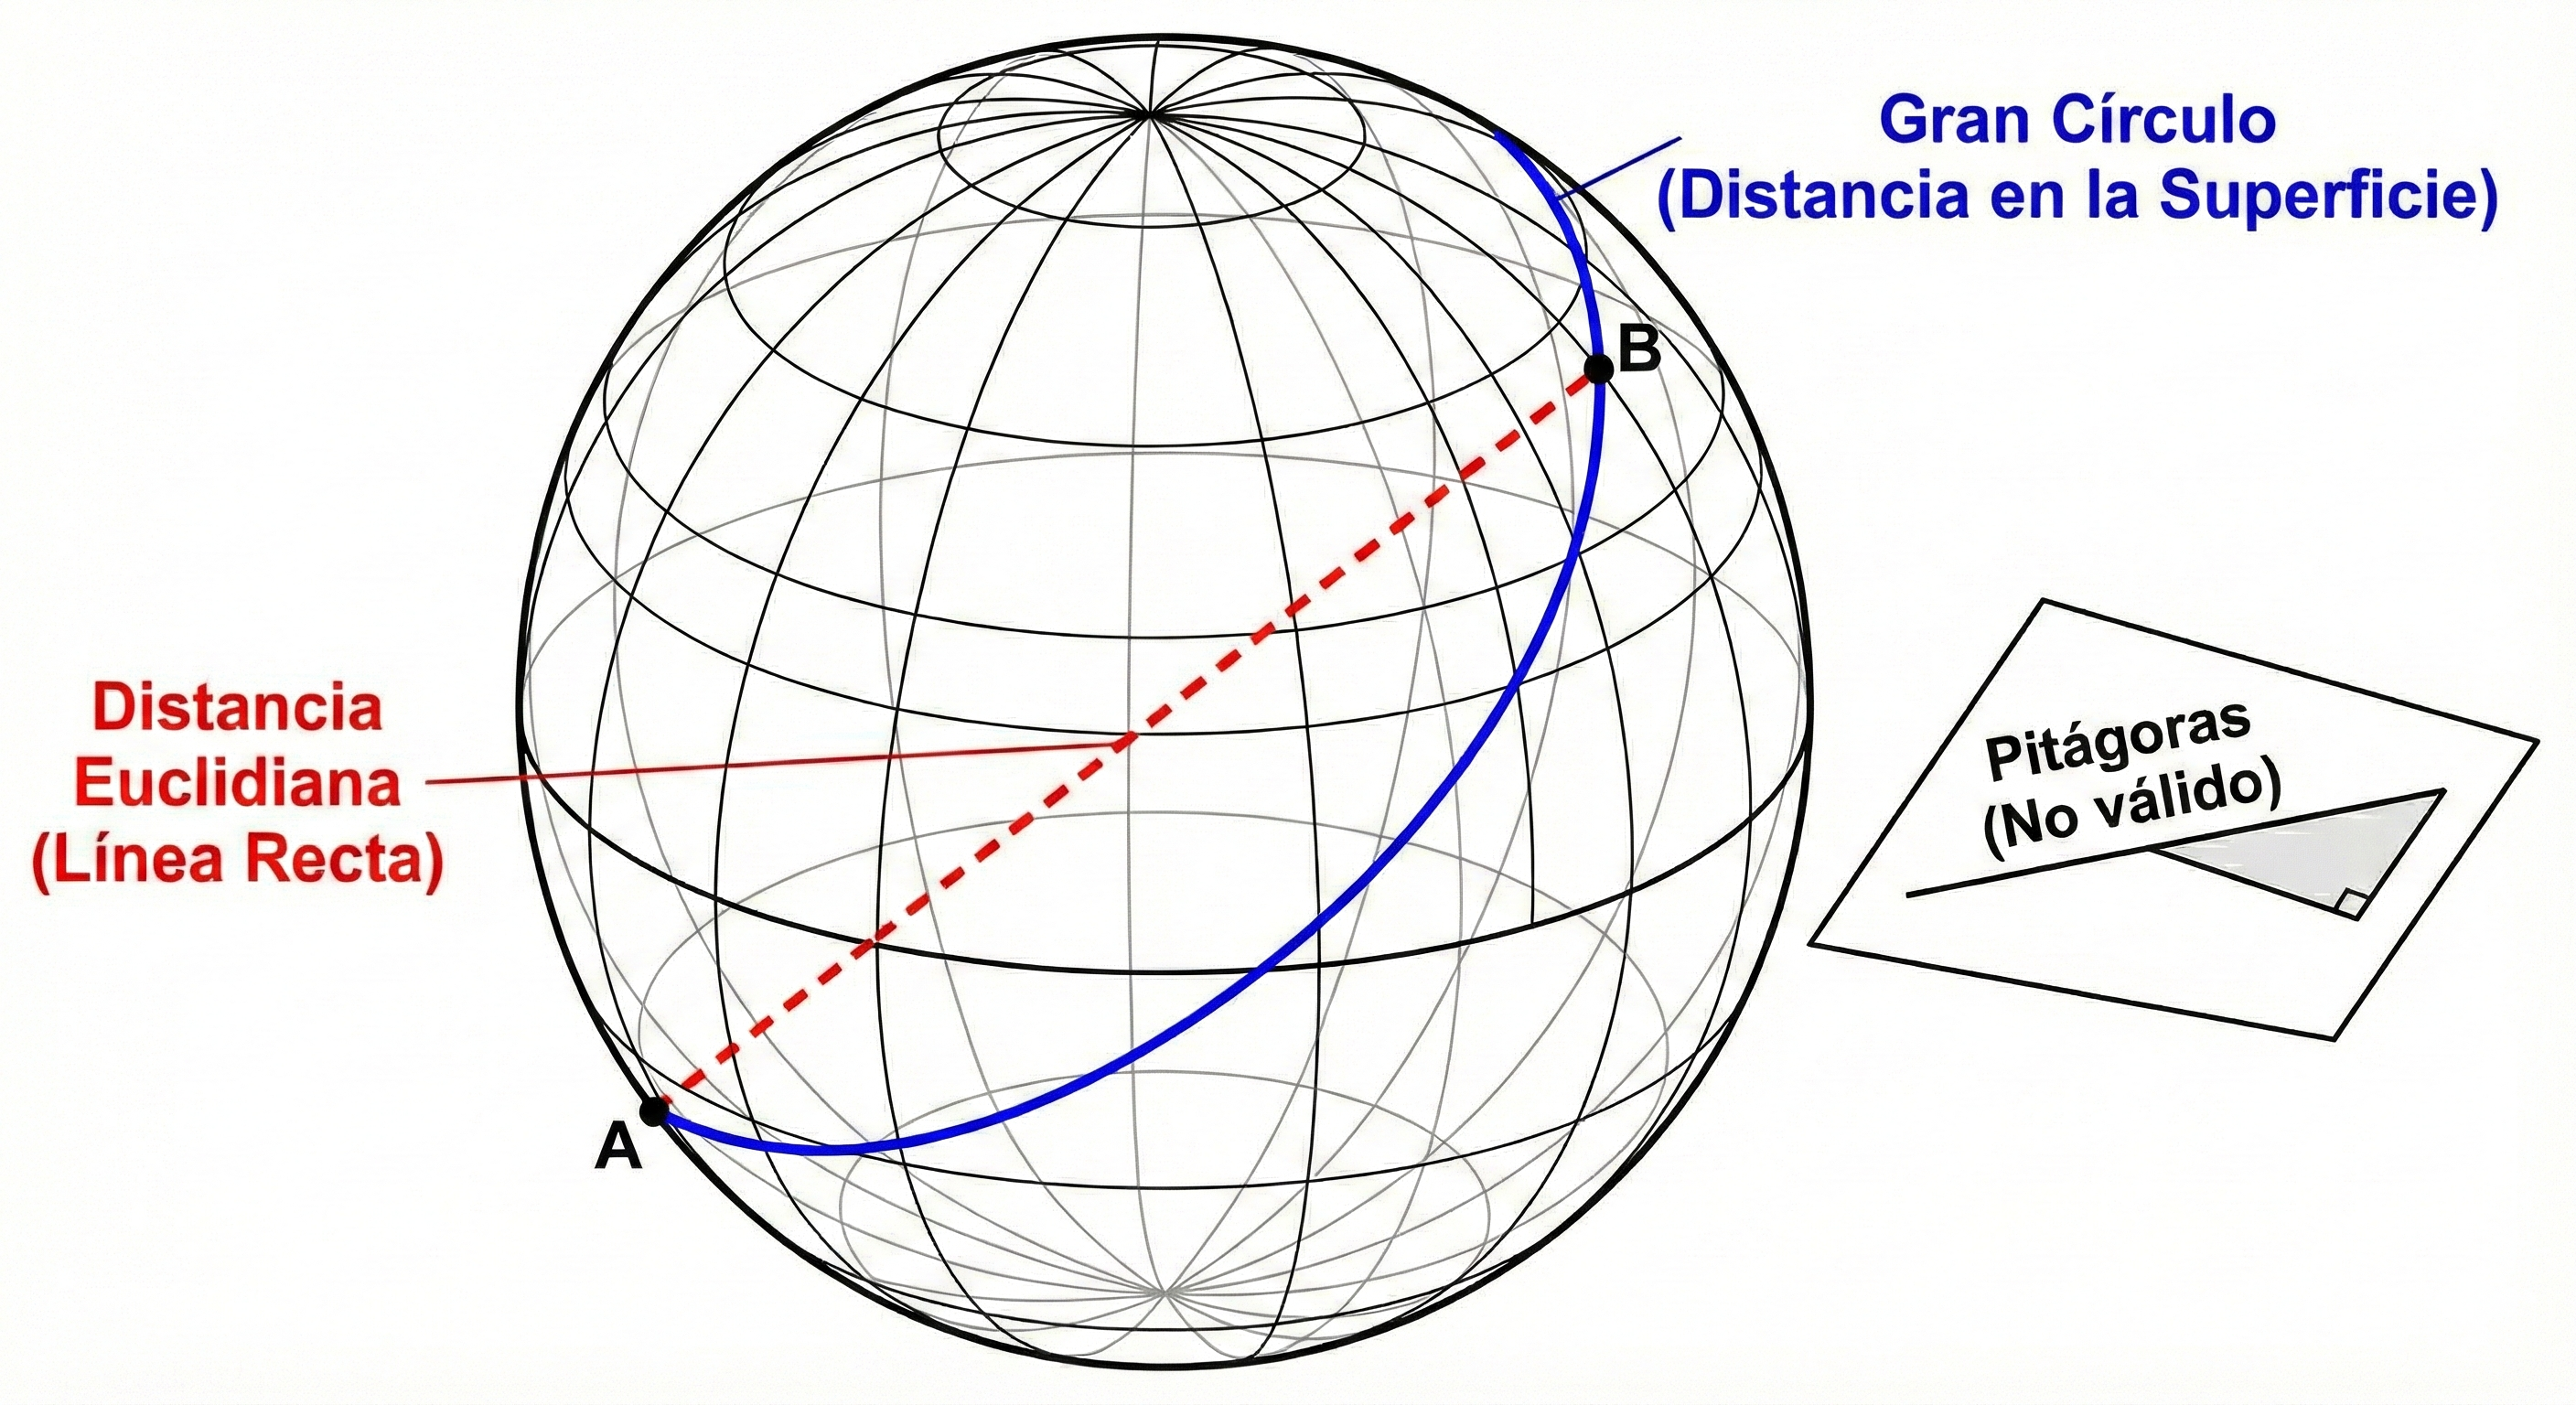
\includegraphics[width=0.6\textwidth,height=\textheight]{./images/great_circle_distance.png}

}

\caption{\label{fig-great_circle}Distancia de Círculo Máximo - fórmula
de Haversine}

\end{figure}%

Matemáticamente, adaptada a las variables de nuestro código, la ecuación
general se ve así:

\[distancia = 2 \cdot radio \cdot \arcsin\left(\sqrt{\sin^2\left(\frac{lat2 - lat1}{2}\right) + \cos(lat1) \cdot \cos(lat2) \cdot \sin^2\left(\frac{lon2 - lon1}{2}\right)}\right)\]

Donde:

\begin{itemize}
\tightlist
\item
  \textbf{\(distancia\)}: Distancia física entre los dos puntos a lo
  largo de la curva de la esfera.
\item
  \textbf{\(radio\)}: Radio de la esfera de referencia (para la Tierra,
  aproximadamente 6371.0 km).
\item
  \textbf{\(lat1\), \(lat2\)}: Latitudes del punto de origen y destino,
  estrictamente en radianes.
\item
  \textbf{\(lon1\), \(lon2\)}: Longitudes del punto de origen y destino,
  estrictamente en radianes.
\end{itemize}

\emph{El truco del radio:} El cálculo trigonométrico interno solo
produce un ángulo sin unidad física (radianes). Para convertirlo en
distancia real, lo multiplicamos por el radio de la Tierra. Si metemos
el radio en kilómetros (6371.0), sale en kilómetros; si lo metemos en
millas (3958.8), sale en millas.

En programación, solemos dividir esta gran fórmula en partes más
pequeñas (las variables \texttt{dlat}, \texttt{dlon}, \texttt{a} y
\texttt{c}) para facilitar la lectura del código y evitar errores,
reemplazando el \(\arcsin\) por la función \texttt{atan2} que es
computacionalmente más estable.

En la práctica, para que el computador procese esta gran ecuación sin
ahogarse (y para evitar errores de paréntesis), los programadores la
dividen en tres pasos secuenciales usando las variables \texttt{a},
\texttt{c} y \texttt{distancia}:

\begin{enumerate}
\def\labelenumi{\arabic{enumi}.}
\item
  \textbf{El ajuste esférico (\(a\)):} Calcula el cuadrado de la mitad
  de la cuerda recta entre los dos puntos.
  \[a = \sin^2\left(\frac{dlat}{2}\right) + \cos(lat1) \cdot \cos(lat2) \cdot \sin^2\left(\frac{dlon}{2}\right)\]
\item
  \textbf{El ángulo central (\(c\)):} Usa la función arcotangente
  (\texttt{atan2}) para hallar el ángulo exacto en radianes desde el
  centro de la Tierra.
  \[c = 2 \cdot \text{atan2}\left(\sqrt{a}, \sqrt{1 - a}\right)\]
\item
  \textbf{La distancia física (\(distancia\)):} Convierte el ángulo en
  una longitud real multiplicándolo por el radio.
  \[distancia = radio \cdot c\]
\end{enumerate}

\begin{tcolorbox}[enhanced jigsaw, title=\textcolor{quarto-callout-note-color}{\faInfo}\hspace{0.5em}{Nota técnica: ¿Por qué usamos atan2 en lugar de arcsin en el código?}, opacityback=0, breakable, colback=white, left=2mm, opacitybacktitle=0.6, colbacktitle=quarto-callout-note-color!10!white, coltitle=black, toptitle=1mm, toprule=.15mm, bottomtitle=1mm, titlerule=0mm, arc=.35mm, rightrule=.15mm, leftrule=.75mm, bottomrule=.15mm, colframe=quarto-callout-note-color-frame]

Si buscas la fórmula matemática clásica de Haversine en un libro,
notarás que utiliza la función arcoseno (\(\arcsin\)). Sin embargo, en
nuestro código de programación usamos la función arcotangente
(\texttt{atan2}). ¿Por qué esta diferencia?

Todo se reduce a la \textbf{precisión computacional (punto flotante)}.
Cuando dos coordenadas están muy cerca la una de la otra, usar
\(\arcsin(\sqrt{a})\) puede generar imprecisiones severas de redondeo en
el procesador.

Para solucionarlo, la programación aprovecha la trigonometría básica
(\(\tan = \frac{\sin}{\cos}\)) usando la función \texttt{atan2(y,\ x)}:

\begin{itemize}
\tightlist
\item
  Sabiendo que \(a = \sin^2\), entonces el seno (cateto opuesto, \(y\))
  es \(\sqrt{a}\).
\item
  Por la regla pitagórica (\(\sin^2 + \cos^2 = 1\)), el coseno (cateto
  adyacente, \(x\)) es \(\sqrt{1 - a}\).
\end{itemize}

Al ingresar
\(c = 2 \cdot \text{atan2}\left(\sqrt{a}, \sqrt{1 - a}\right)\),
obligamos al computador a calcular el ángulo exacto usando ambos lados
del triángulo, garantizando mediciones perfectas ya sea que midamos la
distancia entre dos continentes o entre dos pasos en la calle.

\end{tcolorbox}

Veamos cómo se programan estas máquinas paso a paso, explicando cada
línea de su funcionamiento:

\subsubsection{Python}

\begin{Shaded}
\begin{Highlighting}[]
\CommentTok{\# \#| eval: false}

\CommentTok{\# Importamos la librería matemática nativa de Python para usar senos, cosenos y radianes}
\ImportTok{import}\NormalTok{ math}

\CommentTok{\# {-}{-}{-} FUNCIÓN 1: CÁLCULO MATEMÁTICO BÁSICO {-}{-}{-}}
\KeywordTok{def}\NormalTok{ haversine(lat1, lon1, lat2, lon2, radio}\OperatorTok{=}\FloatTok{6371.0}\NormalTok{):}
    \CommentTok{\# RECIBE: 4 números (lat/lon de dos puntos) y un radio opcional (por defecto 6371.0)}
    
    \CommentTok{\# Convierte la diferencia de latitudes a radianes (el idioma de los computadores)}
\NormalTok{    dlat }\OperatorTok{=}\NormalTok{ math.radians(lat2 }\OperatorTok{{-}}\NormalTok{ lat1)}
    
    \CommentTok{\# Convierte la diferencia de longitudes a radianes}
\NormalTok{    dlon }\OperatorTok{=}\NormalTok{ math.radians(lon2 }\OperatorTok{{-}}\NormalTok{ lon1)}
    
    \CommentTok{\# Calcula \textquotesingle{}a\textquotesingle{}: el cuadrado de la mitad de la cuerda recta entre los puntos}
\NormalTok{    a }\OperatorTok{=}\NormalTok{ (math.sin(dlat }\OperatorTok{/} \DecValTok{2}\NormalTok{) }\OperatorTok{**} \DecValTok{2} \OperatorTok{+} 
\NormalTok{         math.cos(math.radians(lat1)) }\OperatorTok{*}\NormalTok{ math.cos(math.radians(lat2)) }\OperatorTok{*}\NormalTok{ math.sin(dlon }\OperatorTok{/} \DecValTok{2}\NormalTok{) }\OperatorTok{**} \DecValTok{2}\NormalTok{)}
    
    \CommentTok{\# Calcula \textquotesingle{}c\textquotesingle{}: la distancia angular central usando la función arcotangente (atan2)}
\NormalTok{    c }\OperatorTok{=} \DecValTok{2} \OperatorTok{*}\NormalTok{ math.atan2(math.sqrt(a), math.sqrt(}\DecValTok{1} \OperatorTok{{-}}\NormalTok{ a))}
    
    \CommentTok{\# SACA: La multiplicación del ángulo por el radio, dando la distancia física real}
    \ControlFlowTok{return}\NormalTok{ radio }\OperatorTok{*}\NormalTok{ c}

\BuiltInTok{print}\NormalTok{(}\StringTok{"{-}{-}{-} Cálculo de distancia simple {-}{-}{-}"}\NormalTok{)}
\end{Highlighting}
\end{Shaded}

\begin{verbatim}
--- Cálculo de distancia simple ---
\end{verbatim}

\begin{Shaded}
\begin{Highlighting}[]
\CommentTok{\# Ejecutamos la función. Como no le damos el radio, usa el defecto en km.}
\NormalTok{distancia\_km }\OperatorTok{=}\NormalTok{ haversine(}\FloatTok{4.6097}\NormalTok{, }\OperatorTok{{-}}\FloatTok{74.0817}\NormalTok{, }\FloatTok{6.2442}\NormalTok{, }\OperatorTok{{-}}\FloatTok{75.5812}\NormalTok{)}
\BuiltInTok{print}\NormalTok{(}\SpecialStringTok{f"Distancia Bogotá{-}Medellín: }\SpecialCharTok{\{}\NormalTok{distancia\_km}\SpecialCharTok{:.2f\}}\SpecialStringTok{ km"}\NormalTok{)}
\end{Highlighting}
\end{Shaded}

\begin{verbatim}
Distancia Bogotá-Medellín: 246.14 km
\end{verbatim}

\begin{Shaded}
\begin{Highlighting}[]
\CommentTok{\# Sobrescribimos el parámetro \textquotesingle{}radio\textquotesingle{} para obtener el resultado en millas (3958.8)}
\NormalTok{distancia\_millas }\OperatorTok{=}\NormalTok{ haversine(}\FloatTok{4.6097}\NormalTok{, }\OperatorTok{{-}}\FloatTok{74.0817}\NormalTok{, }\FloatTok{6.2442}\NormalTok{, }\OperatorTok{{-}}\FloatTok{75.5812}\NormalTok{, radio}\OperatorTok{=}\FloatTok{3958.8}\NormalTok{)}
\BuiltInTok{print}\NormalTok{(}\SpecialStringTok{f"Distancia en millas: }\SpecialCharTok{\{}\NormalTok{distancia\_millas}\SpecialCharTok{:.2f\}}\SpecialStringTok{ mi"}\NormalTok{)}
\end{Highlighting}
\end{Shaded}

\begin{verbatim}
Distancia en millas: 152.94 mi
\end{verbatim}

\begin{Shaded}
\begin{Highlighting}[]
\CommentTok{\# Aplicamos el "truco" matemático: si le pasamos el radio en metros, el resultado sale en metros}
\NormalTok{distancia\_metros }\OperatorTok{=}\NormalTok{ haversine(}\FloatTok{4.6097}\NormalTok{, }\OperatorTok{{-}}\FloatTok{74.0817}\NormalTok{, }\FloatTok{6.2442}\NormalTok{, }\OperatorTok{{-}}\FloatTok{75.5812}\NormalTok{, radio}\OperatorTok{=}\FloatTok{6371000.0}\NormalTok{)}
\BuiltInTok{print}\NormalTok{(}\SpecialStringTok{f"Distancia en metros: }\SpecialCharTok{\{}\NormalTok{distancia\_metros}\SpecialCharTok{:.2f\}}\SpecialStringTok{ m"}\NormalTok{)}
\end{Highlighting}
\end{Shaded}

\begin{verbatim}
Distancia en metros: 246135.99 m
\end{verbatim}

\begin{Shaded}
\begin{Highlighting}[]
\CommentTok{\# {-}{-}{-} FUNCIÓN 2: PROCESADOR POR LOTES {-}{-}{-}}
\KeywordTok{def}\NormalTok{ medir\_ruta(lista\_coords):}
    \CommentTok{\# RECIBE: Una lista que contiene múltiples tuplas de coordenadas}
    
    \CommentTok{\# Creamos una lista vacía para ir guardando las distancias calculadas}
\NormalTok{    distancias\_tramos }\OperatorTok{=}\NormalTok{ []}
    
    \CommentTok{\# Iniciamos un ciclo que recorre la lista. Paramos un índice antes del final ({-} 1)}
    \CommentTok{\# para no desbordar la lista cuando intentemos buscar el punto \textquotesingle{}i + 1\textquotesingle{}}
    \ControlFlowTok{for}\NormalTok{ i }\KeywordTok{in} \BuiltInTok{range}\NormalTok{(}\BuiltInTok{len}\NormalTok{(lista\_coords) }\OperatorTok{{-}} \DecValTok{1}\NormalTok{):}
        
        \CommentTok{\# Extraemos latitud y longitud del punto actual (donde estamos parados)}
\NormalTok{        lat1, lon1 }\OperatorTok{=}\NormalTok{ lista\_coords[i]}
        
        \CommentTok{\# Extraemos latitud y longitud del punto siguiente (hacia donde vamos)}
\NormalTok{        lat2, lon2 }\OperatorTok{=}\NormalTok{ lista\_coords[i }\OperatorTok{+} \DecValTok{1}\NormalTok{]}
        
        \CommentTok{\# Llamamos a nuestra función \textquotesingle{}haversine\textquotesingle{} para calcular la distancia de este tramo}
\NormalTok{        distancia\_tramo }\OperatorTok{=}\NormalTok{ haversine(lat1, lon1, lat2, lon2)}
        
        \CommentTok{\# Guardamos el resultado de este tramo en nuestra lista final}
\NormalTok{        distancias\_tramos.append(distancia\_tramo)}
        
    \CommentTok{\# SACA: La lista completa con todas las distancias de los tramos calculados}
    \ControlFlowTok{return}\NormalTok{ distancias\_tramos}

\CommentTok{\# Definimos una ruta con 3 puntos (2 tramos)}
\NormalTok{ruta\_colombiana }\OperatorTok{=}\NormalTok{ [(}\FloatTok{4.6097}\NormalTok{, }\OperatorTok{{-}}\FloatTok{74.0817}\NormalTok{), (}\FloatTok{6.2442}\NormalTok{, }\OperatorTok{{-}}\FloatTok{75.5812}\NormalTok{), (}\FloatTok{3.4516}\NormalTok{, }\OperatorTok{{-}}\FloatTok{76.5320}\NormalTok{)]}
\CommentTok{\# Ejecutamos nuestra función procesadora}
\NormalTok{tramos }\OperatorTok{=}\NormalTok{ medir\_ruta(ruta\_colombiana)}

\BuiltInTok{print}\NormalTok{(}\StringTok{"}\CharTok{\textbackslash{}n}\StringTok{{-}{-}{-} Distancia por tramos en una ruta {-}{-}{-}"}\NormalTok{)}
\end{Highlighting}
\end{Shaded}

\begin{verbatim}

--- Distancia por tramos en una ruta ---
\end{verbatim}

\begin{Shaded}
\begin{Highlighting}[]
\CommentTok{\# Imprimimos la lista de resultados usando una comprensión de lista para redondear a 2 decimales}
\BuiltInTok{print}\NormalTok{(}\SpecialStringTok{f"Tramos (km): }\SpecialCharTok{\{}\NormalTok{[}\BuiltInTok{round}\NormalTok{(d, }\DecValTok{2}\NormalTok{) }\ControlFlowTok{for}\NormalTok{ d }\KeywordTok{in}\NormalTok{ tramos]}\SpecialCharTok{\}}\SpecialStringTok{"}\NormalTok{)}
\end{Highlighting}
\end{Shaded}

\begin{verbatim}
Tramos (km): [246.14, 327.9]
\end{verbatim}

\begin{Shaded}
\begin{Highlighting}[]
\CommentTok{\# {-}{-}{-} FUNCIÓN 3: RECOLECTOR DINÁMICO {-}{-}{-}}
\KeywordTok{def}\NormalTok{ describir\_punto(lat, lon, }\OperatorTok{**}\NormalTok{kwargs):}
    \CommentTok{\# RECIBE: Latitud, longitud obligatorias, y un diccionario \textquotesingle{}**kwargs\textquotesingle{} con datos extra inventados}
    
    \CommentTok{\# Iniciamos creando un texto base con las coordenadas obligatorias}
\NormalTok{    descripcion }\OperatorTok{=} \SpecialStringTok{f"Punto (}\SpecialCharTok{\{}\NormalTok{lat}\SpecialCharTok{\}}\SpecialStringTok{, }\SpecialCharTok{\{}\NormalTok{lon}\SpecialCharTok{\}}\SpecialStringTok{)"}
    
    \CommentTok{\# Iniciamos un ciclo para "abrir" el diccionario de parámetros extra.}
    \CommentTok{\# .items() nos separa el nombre de la variable (clave) y su contenido (valor)}
    \ControlFlowTok{for}\NormalTok{ clave, valor }\KeywordTok{in}\NormalTok{ kwargs.items():}
        
        \CommentTok{\# Sumamos al texto base una barrita (|) seguida del nombre y valor del dato extra}
\NormalTok{        descripcion }\OperatorTok{+=} \SpecialStringTok{f" | }\SpecialCharTok{\{}\NormalTok{clave}\SpecialCharTok{\}}\SpecialStringTok{: }\SpecialCharTok{\{}\NormalTok{valor}\SpecialCharTok{\}}\SpecialStringTok{"}
        
    \CommentTok{\# SACA: Un solo texto largo que concatena toda la información del punto}
    \ControlFlowTok{return}\NormalTok{ descripcion}

\BuiltInTok{print}\NormalTok{(}\StringTok{"}\CharTok{\textbackslash{}n}\StringTok{{-}{-}{-} Creación de atributos dinámicos {-}{-}{-}"}\NormalTok{)}
\end{Highlighting}
\end{Shaded}

\begin{verbatim}

--- Creación de atributos dinámicos ---
\end{verbatim}

\begin{Shaded}
\begin{Highlighting}[]
\CommentTok{\# Ejecutamos enviando variables inventadas (ciudad, elevacion, costero, clima)}
\BuiltInTok{print}\NormalTok{(describir\_punto(}\FloatTok{4.6097}\NormalTok{, }\OperatorTok{{-}}\FloatTok{74.0817}\NormalTok{, ciudad}\OperatorTok{=}\StringTok{"Bogotá"}\NormalTok{, elevacion}\OperatorTok{=}\DecValTok{2640}\NormalTok{))}
\end{Highlighting}
\end{Shaded}

\begin{verbatim}
Punto (4.6097, -74.0817) | ciudad: Bogotá | elevacion: 2640
\end{verbatim}

\begin{Shaded}
\begin{Highlighting}[]
\BuiltInTok{print}\NormalTok{(describir\_punto(}\FloatTok{10.3997}\NormalTok{, }\OperatorTok{{-}}\FloatTok{75.4795}\NormalTok{, ciudad}\OperatorTok{=}\StringTok{"Cartagena"}\NormalTok{, costero}\OperatorTok{=}\VariableTok{True}\NormalTok{, clima}\OperatorTok{=}\StringTok{"Cálido"}\NormalTok{))}
\end{Highlighting}
\end{Shaded}

\begin{verbatim}
Punto (10.3997, -75.4795) | ciudad: Cartagena | costero: True | clima: Cálido
\end{verbatim}

\subsubsection{R}

\begin{Shaded}
\begin{Highlighting}[]
\CommentTok{\# \#| eval: false}

\CommentTok{\# R no tiene una función nativa directa para radianes, la creamos rápido}
\NormalTok{pasar\_a\_radianes }\OtherTok{\textless{}{-}} \ControlFlowTok{function}\NormalTok{(grados) \{ }
    \FunctionTok{return}\NormalTok{(grados }\SpecialCharTok{*}\NormalTok{ pi }\SpecialCharTok{/} \DecValTok{180}\NormalTok{) }
\NormalTok{\}}

\CommentTok{\# {-}{-}{-} FUNCIÓN 1: CÁLCULO MATEMÁTICO BÁSICO {-}{-}{-}}
\NormalTok{haversine }\OtherTok{\textless{}{-}} \ControlFlowTok{function}\NormalTok{(lat1, lon1, lat2, lon2, }\AttributeTok{radio =} \FloatTok{6371.0}\NormalTok{) \{}
    \CommentTok{\# RECIBE: 4 coordenadas decimales y un radio opcional (por defecto 6371.0)}
    
    \CommentTok{\# Convierte la diferencia de latitudes a radianes llamando a nuestra mini{-}función}
\NormalTok{    dlat }\OtherTok{\textless{}{-}} \FunctionTok{pasar\_a\_radianes}\NormalTok{(lat2 }\SpecialCharTok{{-}}\NormalTok{ lat1)}
    
    \CommentTok{\# Convierte la diferencia de longitudes a radianes}
\NormalTok{    dlon }\OtherTok{\textless{}{-}} \FunctionTok{pasar\_a\_radianes}\NormalTok{(lon2 }\SpecialCharTok{{-}}\NormalTok{ lon1)}
    
    \CommentTok{\# Calcula \textquotesingle{}a\textquotesingle{}: Ajuste trigonométrico esférico}
\NormalTok{    a }\OtherTok{\textless{}{-}}\NormalTok{ (}\FunctionTok{sin}\NormalTok{(dlat }\SpecialCharTok{/} \DecValTok{2}\NormalTok{)}\SpecialCharTok{\^{}}\DecValTok{2} \SpecialCharTok{+} 
          \FunctionTok{cos}\NormalTok{(}\FunctionTok{pasar\_a\_radianes}\NormalTok{(lat1)) }\SpecialCharTok{*} \FunctionTok{cos}\NormalTok{(}\FunctionTok{pasar\_a\_radianes}\NormalTok{(lat2)) }\SpecialCharTok{*} \FunctionTok{sin}\NormalTok{(dlon }\SpecialCharTok{/} \DecValTok{2}\NormalTok{)}\SpecialCharTok{\^{}}\DecValTok{2}\NormalTok{)}
          
    \CommentTok{\# Calcula \textquotesingle{}c\textquotesingle{}: Ángulo central en radianes usando arcotangente (atan2)}
\NormalTok{    c }\OtherTok{\textless{}{-}} \DecValTok{2} \SpecialCharTok{*} \FunctionTok{atan2}\NormalTok{(}\FunctionTok{sqrt}\NormalTok{(a), }\FunctionTok{sqrt}\NormalTok{(}\DecValTok{1} \SpecialCharTok{{-}}\NormalTok{ a))}
    
    \CommentTok{\# SACA: Multiplica el ángulo por el radio para darnos la distancia física}
\NormalTok{    distancia }\OtherTok{\textless{}{-}}\NormalTok{ radio }\SpecialCharTok{*}\NormalTok{ c}
    \FunctionTok{return}\NormalTok{(distancia) }
\NormalTok{\}}

\FunctionTok{cat}\NormalTok{(}\StringTok{"{-}{-}{-} Cálculo de distancia simple {-}{-}{-}}\SpecialCharTok{\textbackslash{}n}\StringTok{"}\NormalTok{)}
\end{Highlighting}
\end{Shaded}

\begin{verbatim}
--- Cálculo de distancia simple ---
\end{verbatim}

\begin{Shaded}
\begin{Highlighting}[]
\CommentTok{\# Ejecutamos la función usando el radio en kilómetros por defecto}
\NormalTok{distancia\_km }\OtherTok{\textless{}{-}} \FunctionTok{haversine}\NormalTok{(}\FloatTok{4.6097}\NormalTok{, }\SpecialCharTok{{-}}\FloatTok{74.0817}\NormalTok{, }\FloatTok{6.2442}\NormalTok{, }\SpecialCharTok{{-}}\FloatTok{75.5812}\NormalTok{)}
\FunctionTok{cat}\NormalTok{(}\FunctionTok{sprintf}\NormalTok{(}\StringTok{"Distancia Bogotá{-}Medellín: \%.2f km}\SpecialCharTok{\textbackslash{}n}\StringTok{"}\NormalTok{, distancia\_km))}
\end{Highlighting}
\end{Shaded}

\begin{verbatim}
Distancia Bogotá-Medellín: 246.14 km
\end{verbatim}

\begin{Shaded}
\begin{Highlighting}[]
\CommentTok{\# Sobrescribimos el parámetro \textquotesingle{}radio\textquotesingle{} para obtener el resultado en millas (3958.8)}
\NormalTok{distancia\_millas }\OtherTok{\textless{}{-}} \FunctionTok{haversine}\NormalTok{(}\FloatTok{4.6097}\NormalTok{, }\SpecialCharTok{{-}}\FloatTok{74.0817}\NormalTok{, }\FloatTok{6.2442}\NormalTok{, }\SpecialCharTok{{-}}\FloatTok{75.5812}\NormalTok{, }\AttributeTok{radio =} \FloatTok{3958.8}\NormalTok{)}
\FunctionTok{cat}\NormalTok{(}\FunctionTok{sprintf}\NormalTok{(}\StringTok{"Distancia en millas: \%.2f mi}\SpecialCharTok{\textbackslash{}n}\StringTok{"}\NormalTok{, distancia\_millas))}
\end{Highlighting}
\end{Shaded}

\begin{verbatim}
Distancia en millas: 152.94 mi
\end{verbatim}

\begin{Shaded}
\begin{Highlighting}[]
\CommentTok{\# Aplicamos el "truco" matemático: si le pasamos el radio en metros, el resultado sale en metros}
\NormalTok{distancia\_metros }\OtherTok{\textless{}{-}} \FunctionTok{haversine}\NormalTok{(}\FloatTok{4.6097}\NormalTok{, }\SpecialCharTok{{-}}\FloatTok{74.0817}\NormalTok{, }\FloatTok{6.2442}\NormalTok{, }\SpecialCharTok{{-}}\FloatTok{75.5812}\NormalTok{, }\AttributeTok{radio =} \FloatTok{6371000.0}\NormalTok{)}
\FunctionTok{cat}\NormalTok{(}\FunctionTok{sprintf}\NormalTok{(}\StringTok{"Distancia en metros: \%.2f m}\SpecialCharTok{\textbackslash{}n}\StringTok{"}\NormalTok{, distancia\_metros))}
\end{Highlighting}
\end{Shaded}

\begin{verbatim}
Distancia en metros: 246135.99 m
\end{verbatim}

\begin{Shaded}
\begin{Highlighting}[]
\CommentTok{\# {-}{-}{-} FUNCIÓN 2: PROCESADOR POR LOTES {-}{-}{-}}
\NormalTok{medir\_ruta }\OtherTok{\textless{}{-}} \ControlFlowTok{function}\NormalTok{(lista\_coords) \{}
    \CommentTok{\# RECIBE: Una lista de listas numéricas (coordenadas)}
    
    \CommentTok{\# Creamos un vector numérico vacío donde depositaremos las respuestas}
\NormalTok{    distancias\_tramos }\OtherTok{\textless{}{-}} \FunctionTok{c}\NormalTok{() }
    
    \CommentTok{\# Iniciamos el ciclo restando 1 al tamaño total. Si no restamos 1, }
    \CommentTok{\# al final del ciclo R buscará el punto \textquotesingle{}i + 1\textquotesingle{} que no existe y arrojará error.}
    \ControlFlowTok{for}\NormalTok{ (i }\ControlFlowTok{in} \DecValTok{1}\SpecialCharTok{:}\NormalTok{(}\FunctionTok{length}\NormalTok{(lista\_coords) }\SpecialCharTok{{-}} \DecValTok{1}\NormalTok{)) \{}
        
        \CommentTok{\# Extraemos el punto actual (i)}
\NormalTok{        punto\_a }\OtherTok{\textless{}{-}}\NormalTok{ lista\_coords[[i]]}
        
        \CommentTok{\# Extraemos el punto siguiente (i+1)}
\NormalTok{        punto\_b }\OtherTok{\textless{}{-}}\NormalTok{ lista\_coords[[i }\SpecialCharTok{+} \DecValTok{1}\NormalTok{]]}
        
        \CommentTok{\# Llamamos a \textquotesingle{}haversine\textquotesingle{} dándole latitud y longitud de ambos puntos}
\NormalTok{        d }\OtherTok{\textless{}{-}} \FunctionTok{haversine}\NormalTok{(punto\_a[}\DecValTok{1}\NormalTok{], punto\_a[}\DecValTok{2}\NormalTok{], punto\_b[}\DecValTok{1}\NormalTok{], punto\_b[}\DecValTok{2}\NormalTok{])}
        
        \CommentTok{\# Añadimos (concatenamos) la distancia recién calculada a nuestro vector}
\NormalTok{        distancias\_tramos }\OtherTok{\textless{}{-}} \FunctionTok{c}\NormalTok{(distancias\_tramos, d)}
\NormalTok{    \}}
    
    \CommentTok{\# SACA: El vector repleto con las distancias de todos los tramos}
    \FunctionTok{return}\NormalTok{(distancias\_tramos)}
\NormalTok{\}}

\CommentTok{\# Definimos una ruta con 3 puntos (2 tramos)}
\NormalTok{ruta\_colombiana }\OtherTok{\textless{}{-}} \FunctionTok{list}\NormalTok{(}\FunctionTok{c}\NormalTok{(}\FloatTok{4.6097}\NormalTok{, }\SpecialCharTok{{-}}\FloatTok{74.0817}\NormalTok{), }\FunctionTok{c}\NormalTok{(}\FloatTok{6.2442}\NormalTok{, }\SpecialCharTok{{-}}\FloatTok{75.5812}\NormalTok{), }\FunctionTok{c}\NormalTok{(}\FloatTok{3.4516}\NormalTok{, }\SpecialCharTok{{-}}\FloatTok{76.5320}\NormalTok{))}
\CommentTok{\# Ejecutamos la función}
\NormalTok{tramos }\OtherTok{\textless{}{-}} \FunctionTok{medir\_ruta}\NormalTok{(ruta\_colombiana)}

\FunctionTok{cat}\NormalTok{(}\StringTok{"}\SpecialCharTok{\textbackslash{}n}\StringTok{{-}{-}{-} Distancia por tramos en una ruta {-}{-}{-}}\SpecialCharTok{\textbackslash{}n}\StringTok{"}\NormalTok{)}
\end{Highlighting}
\end{Shaded}

\begin{verbatim}

--- Distancia por tramos en una ruta ---
\end{verbatim}

\begin{Shaded}
\begin{Highlighting}[]
\FunctionTok{cat}\NormalTok{(}\FunctionTok{sprintf}\NormalTok{(}\StringTok{"Tramos (km): \%.2f, \%.2f}\SpecialCharTok{\textbackslash{}n}\StringTok{"}\NormalTok{, tramos[}\DecValTok{1}\NormalTok{], tramos[}\DecValTok{2}\NormalTok{]))}
\end{Highlighting}
\end{Shaded}

\begin{verbatim}
Tramos (km): 246.14, 327.90
\end{verbatim}

\begin{Shaded}
\begin{Highlighting}[]
\CommentTok{\# {-}{-}{-} FUNCIÓN 3: RECOLECTOR DINÁMICO {-}{-}{-}}
\NormalTok{describir\_punto }\OtherTok{\textless{}{-}} \ControlFlowTok{function}\NormalTok{(lat, lon, ...) \{}
    \CommentTok{\# RECIBE: lat, lon, y unos tres puntos (...) que atrapan variables extra nombradas}
    
    \CommentTok{\# Creamos el texto base principal}
\NormalTok{    descripcion }\OtherTok{\textless{}{-}} \FunctionTok{sprintf}\NormalTok{(}\StringTok{"Punto (\%.4f, \%.4f)"}\NormalTok{, lat, lon)}
    
    \CommentTok{\# Extraemos las variables atrapadas en los \textquotesingle{}...\textquotesingle{} y las metemos a una lista}
\NormalTok{    args\_extra }\OtherTok{\textless{}{-}} \FunctionTok{list}\NormalTok{(...)}
    
    \CommentTok{\# Verificamos si la lista tiene datos (si el usuario envió algo extra)}
    \ControlFlowTok{if}\NormalTok{ (}\FunctionTok{length}\NormalTok{(args\_extra) }\SpecialCharTok{\textgreater{}} \DecValTok{0}\NormalTok{) \{}
        
        \CommentTok{\# Recorremos cada nombre de variable (clave) en la lista extra}
        \ControlFlowTok{for}\NormalTok{ (clave }\ControlFlowTok{in} \FunctionTok{names}\NormalTok{(args\_extra)) \{}
            
            \CommentTok{\# Pegamos (paste0) la barra, la clave y su valor al texto original}
\NormalTok{            descripcion }\OtherTok{\textless{}{-}} \FunctionTok{paste0}\NormalTok{(descripcion, }\FunctionTok{sprintf}\NormalTok{(}\StringTok{" | \%s: \%s"}\NormalTok{, clave, args\_extra[[clave]]))}
\NormalTok{        \}}
\NormalTok{    \}}
    
    \CommentTok{\# SACA: El texto unificado}
    \FunctionTok{return}\NormalTok{(descripcion)}
\NormalTok{\}}

\FunctionTok{cat}\NormalTok{(}\StringTok{"}\SpecialCharTok{\textbackslash{}n}\StringTok{{-}{-}{-} Creación de atributos dinámicos {-}{-}{-}}\SpecialCharTok{\textbackslash{}n}\StringTok{"}\NormalTok{)}
\end{Highlighting}
\end{Shaded}

\begin{verbatim}

--- Creación de atributos dinámicos ---
\end{verbatim}

\begin{Shaded}
\begin{Highlighting}[]
\CommentTok{\# Pasamos las coordenadas y le inventamos datos (ciudad, elevacion, etc.)}
\FunctionTok{cat}\NormalTok{(}\FunctionTok{describir\_punto}\NormalTok{(}\FloatTok{4.6097}\NormalTok{, }\SpecialCharTok{{-}}\FloatTok{74.0817}\NormalTok{, }\AttributeTok{ciudad=}\StringTok{"Bogotá"}\NormalTok{, }\AttributeTok{elevacion=}\DecValTok{2640}\NormalTok{), }\StringTok{"}\SpecialCharTok{\textbackslash{}n}\StringTok{"}\NormalTok{)}
\end{Highlighting}
\end{Shaded}

\begin{verbatim}
Punto (4.6097, -74.0817) | ciudad: Bogotá | elevacion: 2640 
\end{verbatim}

\begin{Shaded}
\begin{Highlighting}[]
\FunctionTok{cat}\NormalTok{(}\FunctionTok{describir\_punto}\NormalTok{(}\FloatTok{10.3997}\NormalTok{, }\SpecialCharTok{{-}}\FloatTok{75.4795}\NormalTok{, }\AttributeTok{ciudad=}\StringTok{"Cartagena"}\NormalTok{, }\AttributeTok{costero=}\ConstantTok{TRUE}\NormalTok{), }\StringTok{"}\SpecialCharTok{\textbackslash{}n}\StringTok{"}\NormalTok{)}
\end{Highlighting}
\end{Shaded}

\begin{verbatim}
Punto (10.3997, -75.4795) | ciudad: Cartagena | costero: TRUE 
\end{verbatim}

\subsubsection{Julia}

\begin{Shaded}
\begin{Highlighting}[]
\CommentTok{\# \#| eval: false}
\FunctionTok{j\_eval}\NormalTok{(r}\StringTok{"{-}(}
\StringTok{\# {-}{-}{-} FUNCIÓN 1: CÁLCULO MATEMÁTICO BÁSICO {-}{-}{-}}
\StringTok{\# En Julia, los argumentos opcionales con nombre DEBEN ir después de un punto y coma (;)}
\StringTok{function haversine(lat1, lon1, lat2, lon2; radio=6371.0)}
\StringTok{    \# RECIBE: 4 números flotantes y un radio (por defecto en km)}
\StringTok{    }
\StringTok{    \# Convierte la diferencia de latitudes a radianes con la función nativa \textquotesingle{}deg2rad\textquotesingle{}}
\StringTok{    dlat = deg2rad(lat2 {-} lat1)}
\StringTok{    }
\StringTok{    \# Convierte la diferencia de longitudes a radianes}
\StringTok{    dlon = deg2rad(lon2 {-} lon1)}
\StringTok{    }
\StringTok{    \# Calcula \textquotesingle{}a\textquotesingle{}: Ajuste esférico para la Tierra}
\StringTok{    a = (sin(dlat / 2)\^{}2 + }
\StringTok{         cos(deg2rad(lat1)) * cos(deg2rad(lat2)) * sin(dlon / 2)\^{}2)}
\StringTok{         }
\StringTok{    \# Calcula \textquotesingle{}c\textquotesingle{}: Ángulo central en radianes (Ojo: en Julia es solo \textquotesingle{}atan\textquotesingle{}, no \textquotesingle{}atan2\textquotesingle{})}
\StringTok{    c = 2 * atan(sqrt(a), sqrt(1 {-} a)) }
\StringTok{    }
\StringTok{    \# SACA: Multiplica el ángulo por el radio para la distancia real}
\StringTok{    return radio * c}
\StringTok{end}

\StringTok{using Printf}

\StringTok{println("}\SpecialCharTok{{-}{-}{-}}\NormalTok{ Cálculo de distancia simple }\SpecialCharTok{{-}{-}{-}}\StringTok{")}
\StringTok{\# Ejecutamos con el radio por defecto (km)}
\StringTok{distancia\_km = haversine(4.6097, {-}74.0817, 6.2442, {-}75.5812)}
\StringTok{@printf("}\NormalTok{Distancia Bogotá}\SpecialCharTok{{-}}\NormalTok{Medellín}\SpecialCharTok{:}\NormalTok{ \%.}\DecValTok{2}\NormalTok{f km\textbackslash{}n}\StringTok{", distancia\_km)}

\StringTok{\# Sobrescribimos el parámetro \textquotesingle{}radio\textquotesingle{} para obtener el resultado en millas (3958.8)}
\StringTok{distancia\_millas = haversine(4.6097, {-}74.0817, 6.2442, {-}75.5812, radio=3958.8)}
\StringTok{@printf("}\NormalTok{Distancia en millas}\SpecialCharTok{:}\NormalTok{ \%.}\DecValTok{2}\NormalTok{f mi\textbackslash{}n}\StringTok{", distancia\_millas)}

\StringTok{\# Aplicamos el "}\NormalTok{truco}\StringTok{" matemático: si le pasamos el radio en metros, el resultado sale en metros}
\StringTok{distancia\_metros = haversine(4.6097, {-}74.0817, 6.2442, {-}75.5812, radio=6371000.0)}
\StringTok{@printf("}\NormalTok{Distancia en metros}\SpecialCharTok{:}\NormalTok{ \%.}\DecValTok{2}\NormalTok{f m\textbackslash{}n}\StringTok{", distancia\_metros)}


\StringTok{\# {-}{-}{-} FUNCIÓN 2: PROCESADOR POR LOTES {-}{-}{-}}
\StringTok{function medir\_ruta(lista\_coords)}
\StringTok{    \# RECIBE: Un arreglo con tuplas de coordenadas}
\StringTok{    }
\StringTok{    \# Creamos un arreglo vacío pero tipado (Float64) para que Julia procese más rápido}
\StringTok{    distancias\_tramos = Float64[] }
\StringTok{    }
\StringTok{    \# Iniciamos el ciclo restando 1. Si no restamos 1, al final del ciclo}
\StringTok{    \# Julia intentará buscar el punto \textquotesingle{}i + 1\textquotesingle{}, el cual no existe, y colapsará.}
\StringTok{    for i in 1:(length(lista\_coords) {-} 1)}
\StringTok{        }
\StringTok{        \# Extraemos coordenadas iniciales (i) y finales (i+1)}
\StringTok{        lat1, lon1 = lista\_coords[i]}
\StringTok{        lat2, lon2 = lista\_coords[i + 1]}
\StringTok{        }
\StringTok{        \# Invocamos la función \textquotesingle{}haversine\textquotesingle{} y \textquotesingle{}empujamos\textquotesingle{} (push!) el dato al arreglo final}
\StringTok{        push!(distancias\_tramos, haversine(lat1, lon1, lat2, lon2))}
\StringTok{    end}
\StringTok{    }
\StringTok{    \# SACA: Arreglo con las distancias parciales}
\StringTok{    return distancias\_tramos}
\StringTok{end}

\StringTok{\# Definimos una ruta con 3 puntos (2 tramos)}
\StringTok{ruta\_colombiana = [(4.6097, {-}74.0817), (6.2442, {-}75.5812), (3.4516, {-}76.5320)]}
\StringTok{\# Ejecutamos la función}
\StringTok{tramos = medir\_ruta(ruta\_colombiana)}

\StringTok{println("}\NormalTok{\textbackslash{}n}\SpecialCharTok{{-}{-}{-}}\NormalTok{ Distancia por tramos en una ruta }\SpecialCharTok{{-}{-}{-}}\StringTok{")}
\StringTok{@printf("}\FunctionTok{Tramos}\NormalTok{ (km)}\SpecialCharTok{:}\NormalTok{ [}\SpecialCharTok{\%.2f, \%}\NormalTok{.}\DecValTok{2}\NormalTok{f]\textbackslash{}n}\StringTok{", tramos[1], tramos[2])}


\StringTok{\# {-}{-}{-} FUNCIÓN 3: RECOLECTOR DINÁMICO {-}{-}{-}}
\StringTok{\# Usamos \textquotesingle{}kwargs...\textquotesingle{} después del punto y coma (;) para atrapar variables extra con nombre}
\StringTok{function describir\_punto(lat, lon; kwargs...)}
\StringTok{    \# RECIBE: Coordenadas y una "}\NormalTok{bolsa}\StringTok{" con parámetros extra}
\StringTok{    }
\StringTok{    \# Creamos la cadena de texto base}
\StringTok{    descripcion = "}\FunctionTok{Punto}\NormalTok{ (}\SpecialCharTok{$}\NormalTok{lat, }\SpecialCharTok{$}\NormalTok{lon)}\StringTok{"}
\StringTok{    }
\StringTok{    \# Desempaquetamos la bolsa iterando sobre la clave (nombre de variable) y el valor}
\StringTok{    for (clave, valor) in kwargs}
\StringTok{        }
\StringTok{        \# En Julia el operador *= sirve para concatenarle más texto a una cadena existente}
\StringTok{        descripcion *= "} \SpecialCharTok{|} \ErrorTok{$}\NormalTok{clave}\SpecialCharTok{:} \ErrorTok{$}\NormalTok{valor}\StringTok{"}
\StringTok{    end}
\StringTok{    }
\StringTok{    \# SACA: El texto concatenado}
\StringTok{    return descripcion}
\StringTok{end}

\StringTok{println("}\NormalTok{\textbackslash{}n}\SpecialCharTok{{-}{-}{-}}\NormalTok{ Creación de atributos dinámicos }\SpecialCharTok{{-}{-}{-}}\StringTok{")}
\StringTok{\# Le mandamos variables extra (ciudad, elevacion, etc)}
\StringTok{println(describir\_punto(4.6097, {-}74.0817, ciudad="}\NormalTok{Bogotá}\StringTok{", elevacion=2640))}
\StringTok{println(describir\_punto(10.3997, {-}75.4795, ciudad="}\NormalTok{Cartagena}\StringTok{", costero=true))}
\StringTok{){-}"}\NormalTok{)}
\end{Highlighting}
\end{Shaded}

\begin{verbatim}
Starting Julia ...
\end{verbatim}

\subsubsection{Resumen de sintaxis: estructura de
funciones}\label{resumen-de-sintaxis-estructura-de-funciones}

\begin{longtable}[]{@{}
  >{\raggedright\arraybackslash}p{(\columnwidth - 6\tabcolsep) * \real{0.2500}}
  >{\raggedright\arraybackslash}p{(\columnwidth - 6\tabcolsep) * \real{0.2500}}
  >{\raggedright\arraybackslash}p{(\columnwidth - 6\tabcolsep) * \real{0.2500}}
  >{\raggedright\arraybackslash}p{(\columnwidth - 6\tabcolsep) * \real{0.2500}}@{}}
\caption{Diferencias en el empaquetado y argumentos de
funciones}\label{tbl-funciones_argumentos}\tabularnewline
\toprule\noalign{}
\begin{minipage}[b]{\linewidth}\raggedright
Característica
\end{minipage} & \begin{minipage}[b]{\linewidth}\raggedright
Python
\end{minipage} & \begin{minipage}[b]{\linewidth}\raggedright
R
\end{minipage} & \begin{minipage}[b]{\linewidth}\raggedright
Julia
\end{minipage} \\
\midrule\noalign{}
\endfirsthead
\toprule\noalign{}
\begin{minipage}[b]{\linewidth}\raggedright
Característica
\end{minipage} & \begin{minipage}[b]{\linewidth}\raggedright
Python
\end{minipage} & \begin{minipage}[b]{\linewidth}\raggedright
R
\end{minipage} & \begin{minipage}[b]{\linewidth}\raggedright
Julia
\end{minipage} \\
\midrule\noalign{}
\endhead
\bottomrule\noalign{}
\endlastfoot
\textbf{Declaración} & \texttt{def\ calc(x):} &
\texttt{calc\ \textless{}-\ function(x)\ \{\ \}} &
\texttt{function\ calc(x)\ ...\ end} \\
\textbf{Retorno} & \texttt{return\ y} & \texttt{return(y)} &
\texttt{return\ y} \\
\textbf{Parámetro x defecto} & \texttt{def\ calc(r=6371):} &
\texttt{function(r=6371)} & \texttt{function\ calc(;\ r=6371)} \\
\textbf{Múltiples args extra} & \texttt{**kwargs} & \texttt{...} &
\texttt{kwargs...} \\
\end{longtable}

\subsection{2. Clases: organizando datos y comportamiento
juntos}\label{clases-organizando-datos-y-comportamiento-juntos}

En el mundo del desarrollo de software, existen diferentes formas de
estructurar el código. Tradicionalmente, la programación separaba los
datos por un lado y las funciones que operaban sobre esos datos por el
otro. Sin embargo, la \textbf{Programación Orientada a Objetos (POO)}
propone un paradigma distinto: agrupar los datos y los comportamientos
relacionados en una sola entidad unificada.

Para dominar este paradigma, primero debemos entender sus conceptos
genéricos fundamentales:

\begin{itemize}
\tightlist
\item
  \textbf{Clase:} Es el plano, la plantilla o el molde abstracto. No
  contiene datos reales, sino que define qué estructura tendrán los
  datos y qué acciones se podrán realizar.
\item
  \textbf{Objeto (o instancia):} Es la materialización de la clase. Es
  el producto final creado a partir del molde, que ocupa un espacio real
  en la memoria de la computadora y contiene datos específicos.
\item
  \textbf{Atributos (o estado):} Son las variables internas que guardan
  las características únicas de cada objeto.
\item
  \textbf{Métodos (o comportamiento):} Son las funciones que viven
  dentro (o asociadas) al objeto. Definen lo que el objeto ``sabe
  hacer'' con sus propios datos.
\item
  \textbf{Constructor:} Es la puerta de entrada. Es el mecanismo inicial
  que toma los datos crudos y los ensambla siguiendo las reglas de la
  clase para dar vida a un nuevo objeto.
\end{itemize}

\subsubsection{Analogía entre clases/objetos y
moldes/arepas}\label{analoguxeda-entre-clasesobjetos-y-moldesarepas}

\begin{itemize}
\tightlist
\item
  \textbf{La Clase (el molde):} Es como el plano arquitectónico de una
  casa o el molde para hacer arepas. El molde define que toda arepa
  tendrá un grosor y un diámetro, pero el molde en sí no se puede comer.
\item
  \textbf{El Objeto (la instancia):} Es la arepa ya hecha, salida del
  molde. Puedes sacar mil arepas distintas (unas de queso, otras de
  carne) usando el mismo molde. Todas comparten la misma estructura,
  pero contienen datos (rellenos) diferentes.
\end{itemize}

\subsubsection{El reto: de simples números a entidades
inteligentes}\label{el-reto-de-simples-nuxfameros-a-entidades-inteligentes}

En el análisis de datos espaciales, solemos trabajar con coordenadas
crudas (simples pares de números). Si los dejamos sueltos, son solo
texto sin significado. Nuestro objetivo en este ejercicio es aplicar los
conceptos de la POO para tomar esos números y ``darles vida''.

Queremos tomar dos simples coordenadas geográficas y convertirlas en un
\textbf{Objeto Espacial Inteligente} que tenga la capacidad intrínseca
de realizar tres tareas fundamentales:

\begin{enumerate}
\def\labelenumi{\arabic{enumi}.}
\tightlist
\item
  \textbf{Representarse a sí mismo (Texto):} Que el objeto pueda
  decirnos su nombre y ubicación en un formato legible para humanos.
\item
  \textbf{Analítica espacial (Matemáticas):} Que el objeto tenga la
  capacidad de calcular la distancia hacia otro punto.
\item
  \textbf{Visualización (Gráficos):} Que el objeto, al recibir un punto
  de destino, sepa cómo dibujar un mapa interactivo mostrando la ruta y
  la distancia entre ambos.
\end{enumerate}

A continuación, ilustramos conceptualmente este flujo de transformación:

\begin{figure}

\centering{

\includegraphics{./images/ejercicio_clases.png}

}

\caption{\label{fig-flujo-conceptual}Flujo conceptual: Transformación de
datos crudos en un objeto inteligente con capacidades.}

\end{figure}%

En esta sección, crearemos una Clase llamada \texttt{PuntoEspacial}.
Este ``molde'' le enseñará a la computadora cuatro cosas fundamentales:

\subsubsection{Python y la Programación Orientada a Objetos
(OOP)}\label{python-y-la-programaciuxf3n-orientada-a-objetos-oop}

En Python, la creación de estructuras de datos y su comportamiento sigue
un enfoque clásico y estricto de \textbf{Programación Orientada a
Objetos (OOP)}. A diferencia de otros lenguajes donde los datos y las
funciones operan por separado, Python prefiere encapsularlo todo (el
estado y las acciones) dentro de una única fortaleza lógica: \textbf{La
Clase}.

\begin{tcolorbox}[enhanced jigsaw, title=\textcolor{quarto-callout-tip-color}{\faLightbulb}\hspace{0.5em}{La Analogía: El Molde y la Arepa}, opacityback=0, breakable, colback=white, left=2mm, opacitybacktitle=0.6, colbacktitle=quarto-callout-tip-color!10!white, coltitle=black, toptitle=1mm, toprule=.15mm, bottomtitle=1mm, titlerule=0mm, arc=.35mm, rightrule=.15mm, leftrule=.75mm, bottomrule=.15mm, colframe=quarto-callout-tip-color-frame]

Para visualizar cómo Python maneja la memoria, imaginemos una cocina:

\begin{itemize}
\tightlist
\item
  \textbf{La Clase (\texttt{class\ PuntoEspacial}):} Es el \textbf{molde
  de hierro}. Por sí solo no contiene ingredientes ni alimenta a nadie;
  es simplemente un diseño estático que dicta la estructura geométrica,
  qué datos son obligatorios y qué acciones se pueden realizar.
\item
  \textbf{El Objeto (La Instancia):} Es la \textbf{arepa física y
  calientita}. Cuando pasamos ingredientes reales (latitud, longitud,
  nombre) a través del molde, el computador reserva un espacio en
  memoria para crear una instancia concreta y única. Podemos sacar mil
  ``arepas'' (objetos) del mismo molde, y cada una tendrá sus propios
  datos independientes.
\end{itemize}

\end{tcolorbox}

\paragraph{La anatomía del molde}\label{la-anatomuxeda-del-molde}

Cuando diseñamos una clase en Python, establecemos un contrato estricto
con la máquina a través de métodos mágicos y atributos:

\begin{enumerate}
\def\labelenumi{\arabic{enumi}.}
\item
  \textbf{El Constructor (\texttt{\_\_init\_\_}):} Es la puerta de
  entrada. Cada vez que intentamos crear un objeto nuevo, Python llama
  automáticamente a esta función para recibir los parámetros iniciales y
  ``ensamblar'' la estructura en la memoria.
\item
  \textbf{El Auto-reconocimiento (\texttt{self}):} En Python, la clase
  necesita una forma de referirse a la ``arepa'' específica que está
  cocinando en ese momento. El parámetro \texttt{self} es ese ancla;
  garantiza que si modificamos la latitud del ``Punto A'', no
  estropeemos accidentalmente la latitud del ``Punto B''.
\item
  \textbf{La representación (\texttt{\_\_str\_\_}):} Cómo debe
  presentarse el objeto si intentamos imprimirlo en pantalla.
\item
  \textbf{Los Métodos (Comportamiento):} Son las funciones que viven
  \textbf{dentro} de la clase. Una vez instanciado el objeto, este carga
  consigo mismo todas sus herramientas. Un punto espacial en Python
  ``sabe'' cómo calcular su propia distancia hacia otro punto o cómo
  graficarse a sí mismo en un mapa.

  \begin{itemize}
  \tightlist
  \item
    \textbf{Los métodos analíticos (\texttt{distancia\_hacia}):}
    Funciones que viven \emph{dentro} del objeto. Nuestro punto será tan
    inteligente que sabrá calcular la distancia hacia otro punto por sí
    mismo, invocando internamente a la función \texttt{haversine} que
    programamos en la sección anterior. Además, le agregaremos un
    parámetro dinámico para que pueda devolver la distancia en
    \textbf{metros} si se lo pedimos.
  \item
    \textbf{El método gráfico (\texttt{graficar\_ruta}):} Un método que
    le permite al objeto usar una librería cartográfica para dibujarse a
    sí mismo en un mapa base. Además, usaremos nuestro método analítico
    para calcular el punto medio y ¡escribir la distancia calculada
    directamente sobre la línea de la ruta!
  \end{itemize}
\end{enumerate}

A continuación, visualizamos este ciclo de vida completo: primero, el
diagrama estructural del molde (la Clase) y sus métodos internos; y
luego, el mapa de ejecución que muestra cómo sacamos las instancias
(Objetos) a la memoria para interactuar con ellas.

\begin{figure}

\centering{

\includegraphics{./images/clase_python.png}

}

\caption{\label{fig-clases-python-final-vertical}Diagrama del flujo de
instanciación: El molde (Clase) y las arepas (Objetos).}

\end{figure}%

\begin{figure}

\centering{

\includegraphics{./images/clase_python_codigo.png}

}

\caption{\label{fig-clases-python-codigo}Ejecución del código
instanciando los objetos en memoria.}

\end{figure}%

\subsubsection{R y el sistema S3: la ilusión del molde y el poder de la
etiqueta}\label{r-y-el-sistema-s3-la-ilusiuxf3n-del-molde-y-el-poder-de-la-etiqueta}

Mientras que Python utiliza un enfoque estricto donde cada objeto nace
de un ``molde de hierro'' predefinido, R aborda la programación
orientada a objetos de una manera mucho más relajada e informal,
principalmente a través de su \textbf{sistema S3}.

En R, las clases no se definen formalmente. No hay una bóveda blindada
que encierre los datos y los métodos juntos. En su lugar, el sistema S3
confía en el ``sistema de honor'' y en el uso inteligente de etiquetas.

\begin{tcolorbox}[enhanced jigsaw, title=\textcolor{quarto-callout-note-color}{\faInfo}\hspace{0.5em}{La analogía: el recipiente común y el post-it}, opacityback=0, breakable, colback=white, left=2mm, opacitybacktitle=0.6, colbacktitle=quarto-callout-note-color!10!white, coltitle=black, toptitle=1mm, toprule=.15mm, bottomtitle=1mm, titlerule=0mm, arc=.35mm, rightrule=.15mm, leftrule=.75mm, bottomrule=.15mm, colframe=quarto-callout-note-color-frame]

Si en Python teníamos un molde de hierro para hacer arepas, en R la
cocina funciona muy distinto:

\begin{itemize}
\tightlist
\item
  \textbf{Los ingredientes (la lista):} En lugar de un molde, tomamos un
  recipiente plástico común y corriente (como el ``porta'' del almuerzo
  o una \texttt{list} en R), y echamos ahí nuestros ingredientes crudos
  (latitud, longitud y nombre).
\item
  \textbf{La ``clase'' (el post-it):} Para convertir esa lista genérica
  en un objeto espacial, literalmente le pegamos un ``post-it'' en la
  tapa del recipiente. Al asignarle un atributo de clase
  (\texttt{class(objeto)\ \textless{}-\ \textquotesingle{}PuntoEspacial\textquotesingle{}}),
  le estamos diciendo a R: \emph{``De ahora en adelante, confía en mí y
  trata a este recipiente como si fuera una arepa''}.
\end{itemize}

\end{tcolorbox}

\paragraph{La anatomía del sistema
S3}\label{la-anatomuxeda-del-sistema-s3}

Dado que no hay un ``molde'' real, la instanciación y el comportamiento
en R se dividen en tres pilares fundamentales que flotan libremente en
el entorno:

\begin{enumerate}
\def\labelenumi{\arabic{enumi}.}
\tightlist
\item
  \textbf{El constructor informal:} Es simplemente una función normal
  (como \texttt{nuevo\_punto\_espacial()}) que recibe los datos, los
  empaqueta en una lista y, lo más importante, le estampa la etiqueta de
  la clase antes de devolverla.
\item
  \textbf{Las funciones genéricas (los inspectores):} Funciones como
  \texttt{print()} o \texttt{distancia\_hacia()} son genéricas. No saben
  cómo calcular nada por sí mismas; su único trabajo es mirar el
  ``post-it'' del objeto que reciben y decir: \emph{``Ah, eres un
  PuntoEspacial, déjame buscar al experto que sabe tratar contigo''}.
  Esto se logra mediante el comando interno \texttt{UseMethod()}.
\item
  \textbf{Los métodos específicos (el despacho):} Son las funciones que
  realmente hacen el trabajo duro, y se nombran uniendo el genérico y la
  clase (por ejemplo, \texttt{distancia\_hacia.PuntoEspacial()}). El
  genérico le ``despacha'' el objeto a esta función especializada.
\end{enumerate}

A continuación, visualizamos este paradigma en acción: primero, el
diagrama arquitectónico que muestra cómo los métodos flotan fuera de la
estructura de datos; y luego, el bloque de ejecución donde vemos la
magia del etiquetado y el despacho S3 en tiempo real.

\begin{figure}

\centering{

\includegraphics{./images/clase_r.png}

}

\caption{\label{fig-clases-r-final-vertical}Diagrama del flujo de
instanciación en R (S3): El molde y las arepas.}

\end{figure}%

\begin{figure}

\centering{

\includegraphics{./images/clase_r_codigo.png}

}

\caption{\label{fig-clases-r-codigo}Ejecución del código en R (S3)
instanciando los objetos en memoria.}

\end{figure}%

\subsubsection{Julia y el despacho múltiple: separando los ingredientes
de la
receta}\label{julia-y-el-despacho-muxfaltiple-separando-los-ingredientes-de-la-receta}

Julia rechaza por completo el concepto tradicional de clases que vimos
en Python. En su lugar, abraza un paradigma donde los datos (las
variables) y el comportamiento (las funciones) están estrictamente
separados, pero trabajan en una armonía perfecta gracias al núcleo
absoluto del lenguaje: el \textbf{despacho múltiple} (Multiple
Dispatch).

\begin{tcolorbox}[enhanced jigsaw, title=\textcolor{quarto-callout-tip-color}{\faLightbulb}\hspace{0.5em}{La analogía: el contenedor rígido y los chefs expertos}, opacityback=0, breakable, colback=white, left=2mm, opacitybacktitle=0.6, colbacktitle=quarto-callout-tip-color!10!white, coltitle=black, toptitle=1mm, toprule=.15mm, bottomtitle=1mm, titlerule=0mm, arc=.35mm, rightrule=.15mm, leftrule=.75mm, bottomrule=.15mm, colframe=quarto-callout-tip-color-frame]

Si Python es un molde de hierro y R es un post-it, Julia es una cocina
de alta eficiencia:

\begin{itemize}
\tightlist
\item
  \textbf{El contenedor (\texttt{struct}):} Es un contenedor plástico
  rígido (como un ``porta'' de cristal). Su única función es guardar los
  ingredientes (latitud, longitud, nombre) de forma organizada y con
  etiquetas de tipo muy estrictas (\texttt{Float64}, \texttt{String}).
  El \texttt{struct} es ``tonto''; no sabe hacer absolutamente nada por
  sí solo, no tiene métodos ni recetas grabadas en sus paredes.
\item
  \textbf{El comportamiento (las funciones libres):} Son un batallón de
  chefs expertos que están esperando en la cocina. Cuando usted grita
  ``¡Quiero la distancia!'', el jefe de cocina (el compilador de Julia)
  mira exactamente qué ingredientes le entregó en el porta. Dependiendo
  de los tipos de datos que usted mande, le asigna el trabajo al chef
  que tenga la receta matemática más optimizada para esos tipos exactos.
\end{itemize}

\end{tcolorbox}

\paragraph{La anatomía de la arquitectura en
Julia}\label{la-anatomuxeda-de-la-arquitectura-en-julia}

En este lenguaje, construimos la estructura definiendo tipos de datos
crudos y luego escribimos funciones libres que declaran para qué
combinaciones de tipos están preparadas.

\begin{enumerate}
\def\labelenumi{\arabic{enumi}.}
\tightlist
\item
  \textbf{La estructura base (\texttt{struct}):} A diferencia de las
  clases, aquí solo organizamos las variables en la memoria. Esto
  garantiza un tipado fuerte que le permite a Julia ser tan rápido como
  C o Fortran.
\item
  \textbf{El constructor:} Julia crea un constructor automático básico,
  pero podemos crear constructores propios si necesitamos reglas
  especiales (como asignar `no name' si el usuario olvida el nombre al
  llenar el contenedor).
\item
  \textbf{El despacho múltiple en acción:} La magia ocurre al llamar a
  una función. Si tenemos una función \texttt{distancia\_hacia(a,\ b)},
  Julia analiza el tipo de dato exacto de \textbf{todos} los argumentos
  que le pasamos. Basado en esa combinación de tipos, el lenguaje enruta
  la ejecución al método más específico de forma instantánea.
\end{enumerate}

A continuación, visualizamos este potente paradigma: primero, la
representación de cómo el \texttt{struct} y el despacho múltiple
interactúan conceptualmente en una ``caja virtual'' (con líneas muy
espaciadas para notar que no es una prisión de código); y luego, el
bloque de ejecución donde vemos a Julia activando los métodos correctos
al vuelo.

\begin{figure}

\centering{

\includegraphics{./images/clase_julia.png}

}

\caption{\label{fig-clases-julia-final-vertical}Diagrama del flujo de
instanciación en Julia (Despacho Múltiple): El molde (Struct) y las
arepas.}

\end{figure}%

\begin{figure}

\centering{

\includegraphics{./images/clase_julia_codigo.png}

}

\caption{\label{fig-clases-julia-codigo}Ejecución del código en Julia
instanciando las estructuras en memoria.}

\end{figure}%

\subsubsection{Laboratorio comparativo: implementación del código
completo}\label{laboratorio-comparativo-implementaciuxf3n-del-cuxf3digo-completo}

A continuación, presentamos el código completo y funcional para los tres
lenguajes. Te invitamos a navegar entre las pestañas para comparar cómo
cada arquitectura resuelve el mismo problema.

💡 \textbf{Tip de lectura:} Busca las etiquetas con emojis
(\texttt{{[}1\ 📍{]}}, \texttt{{[}2\ 💬{]}}, \texttt{{[}3\ 📐{]}},
\texttt{{[}4\ 🗺️📐{]}}) dentro de los comentarios del código. Estas te
ayudarán a conectar cada bloque de código directamente con los diagramas
de arquitectura que vimos en las secciones anteriores.

\paragraph{Python}

\begin{Shaded}
\begin{Highlighting}[]
\CommentTok{\# \#| echo: false}
\CommentTok{\# \#| eval: false}
\ImportTok{import}\NormalTok{ math}
\ImportTok{import}\NormalTok{ folium }\CommentTok{\# Librería indispensable en Python para generar mapas interactivos}

\CommentTok{\# {-}{-}{-} 0. TRAEMOS NUESTRA MÁQUINA MATEMÁTICA {-}{-}{-}}
\CommentTok{\# Pegamos aquí la función que ya habíamos creado para que este código funcione por sí solo}
\KeywordTok{def}\NormalTok{ haversine(lat1, lon1, lat2, lon2, radio}\OperatorTok{=}\FloatTok{6371.0}\NormalTok{):}
\NormalTok{    dlat, dlon }\OperatorTok{=}\NormalTok{ math.radians(lat2 }\OperatorTok{{-}}\NormalTok{ lat1), math.radians(lon2 }\OperatorTok{{-}}\NormalTok{ lon1)}
\NormalTok{    a }\OperatorTok{=}\NormalTok{ math.sin(dlat }\OperatorTok{/} \DecValTok{2}\NormalTok{)}\OperatorTok{**}\DecValTok{2} \OperatorTok{+}\NormalTok{ math.cos(math.radians(lat1)) }\OperatorTok{*}\NormalTok{ math.cos(math.radians(lat2)) }\OperatorTok{*}\NormalTok{ math.sin(dlon }\OperatorTok{/} \DecValTok{2}\NormalTok{)}\OperatorTok{**}\DecValTok{2}
    \ControlFlowTok{return}\NormalTok{ radio }\OperatorTok{*}\NormalTok{ (}\DecValTok{2} \OperatorTok{*}\NormalTok{ math.atan2(math.sqrt(a), math.sqrt(}\DecValTok{1} \OperatorTok{{-}}\NormalTok{ a)))}


\CommentTok{\# {-}{-}{-} 1. DEFINICIÓN DEL MOLDE (LA CLASE) {-}{-}{-}}
\CommentTok{\# Usamos la palabra reservada \textquotesingle{}class\textquotesingle{} seguida del nombre (en mayúscula por convención)}
\KeywordTok{class}\NormalTok{ PuntoEspacial:}
    
    \CommentTok{\# [1 📍] 1.1 EL CONSTRUCTOR (\_\_init\_\_)}
    \CommentTok{\# Esta función especial se ejecuta automáticamente el momento en que "nace" un punto.}
    \CommentTok{\# \textquotesingle{}self\textquotesingle{} significa "yo mismo". Es la forma en que el objeto se refiere a sus propios datos.}
    \CommentTok{\# Definimos que latitud y longitud son obligatorios, pero el nombre tiene un valor por defecto.}
    \KeywordTok{def} \FunctionTok{\_\_init\_\_}\NormalTok{(}\VariableTok{self}\NormalTok{, latitud, longitud, nombre}\OperatorTok{=}\StringTok{"Punto sin nombre"}\NormalTok{):}
        
        \CommentTok{\# Guardamos la latitud que nos entregaron dentro del cuerpo del objeto (self)}
        \VariableTok{self}\NormalTok{.latitud }\OperatorTok{=}\NormalTok{ latitud}
        
        \CommentTok{\# Guardamos la longitud dentro del objeto}
        \VariableTok{self}\NormalTok{.longitud }\OperatorTok{=}\NormalTok{ longitud}
        
        \CommentTok{\# Guardamos el nombre dentro del objeto}
        \VariableTok{self}\NormalTok{.nombre }\OperatorTok{=}\NormalTok{ nombre}

    \CommentTok{\# [2 💬] 1.2 LA REPRESENTACIÓN TEXTUAL (\_\_str\_\_)}
    \CommentTok{\# Si le decimos a Python print(objeto), por defecto imprimirá basura técnica.}
    \CommentTok{\# Esta función especial le enseña a Python cómo queremos que se lea el objeto en pantalla.}
    \KeywordTok{def} \FunctionTok{\_\_str\_\_}\NormalTok{(}\VariableTok{self}\NormalTok{):}
        \CommentTok{\# SACA: Un texto bonito combinando el nombre y las coordenadas}
        \ControlFlowTok{return} \SpecialStringTok{f"[}\SpecialCharTok{\{}\VariableTok{self}\SpecialCharTok{.}\NormalTok{nombre}\SpecialCharTok{\}}\SpecialStringTok{] (Lat: }\SpecialCharTok{\{}\VariableTok{self}\SpecialCharTok{.}\NormalTok{latitud}\SpecialCharTok{\}}\SpecialStringTok{, Lon: }\SpecialCharTok{\{}\VariableTok{self}\SpecialCharTok{.}\NormalTok{longitud}\SpecialCharTok{\}}\SpecialStringTok{)"}

    \CommentTok{\# [3 📐] 1.3 LOS MÉTODOS (COMPORTAMIENTO ANALÍTICO)}
    \CommentTok{\# Es una función normal, pero como tiene \textquotesingle{}self\textquotesingle{}, vive dentro del objeto.}
    \CommentTok{\# Agregamos el parámetro \textquotesingle{}radio\textquotesingle{} para que el usuario pueda pedir el resultado en metros.}
    \KeywordTok{def}\NormalTok{ distancia\_hacia(}\VariableTok{self}\NormalTok{, otro\_punto, radio}\OperatorTok{=}\FloatTok{6371.0}\NormalTok{):}
        
        \CommentTok{\# Llamamos a nuestra función haversine externa pasándole el radio solicitado}
        \CommentTok{\# Le enviamos NUESTRAS coordenadas (self) y las coordenadas DEL OTRO (otro\_punto)}
\NormalTok{        distancia }\OperatorTok{=}\NormalTok{ haversine(}\VariableTok{self}\NormalTok{.latitud, }\VariableTok{self}\NormalTok{.longitud, otro\_punto.latitud, otro\_punto.longitud, radio)}
        
        \CommentTok{\# SACA: La distancia numérica calculada entre los dos objetos}
        \ControlFlowTok{return}\NormalTok{ distancia}
        
    \CommentTok{\# [4 🗺️📐] 1.4 EL MÉTODO GRÁFICO (MAPA BASE CON ETIQUETA VISIBLE)}
    \CommentTok{\# Este método le da la habilidad al objeto de dibujarse en un mapa web interactivo.}
    \KeywordTok{def}\NormalTok{ graficar\_ruta(}\VariableTok{self}\NormalTok{, otro\_punto):}
        
        \CommentTok{\# Primero, le decimos al objeto que calcule su propia distancia hacia el destino}
\NormalTok{        distancia\_calculada }\OperatorTok{=} \VariableTok{self}\NormalTok{.distancia\_hacia(otro\_punto)}
        
        \CommentTok{\# Calculamos el punto medio geométrico para centrar la cámara y poner el texto}
\NormalTok{        centro\_lat }\OperatorTok{=}\NormalTok{ (}\VariableTok{self}\NormalTok{.latitud }\OperatorTok{+}\NormalTok{ otro\_punto.latitud) }\OperatorTok{/} \DecValTok{2}
\NormalTok{        centro\_lon }\OperatorTok{=}\NormalTok{ (}\VariableTok{self}\NormalTok{.longitud }\OperatorTok{+}\NormalTok{ otro\_punto.longitud) }\OperatorTok{/} \DecValTok{2}
        
        \CommentTok{\# Creamos el lienzo del mapa base (estilo OpenStreetMap por defecto)}
\NormalTok{        mapa }\OperatorTok{=}\NormalTok{ folium.Map(location}\OperatorTok{=}\NormalTok{[centro\_lat, centro\_lon], zoom\_start}\OperatorTok{=}\DecValTok{6}\NormalTok{)}
        
        \CommentTok{\# Ponemos un pin en nuestra ubicación de origen (self)}
\NormalTok{        folium.Marker([}\VariableTok{self}\NormalTok{.latitud, }\VariableTok{self}\NormalTok{.longitud], popup}\OperatorTok{=}\VariableTok{self}\NormalTok{.nombre).add\_to(mapa)}
        
        \CommentTok{\# Ponemos un pin en el destino (otro\_punto)}
\NormalTok{        folium.Marker([otro\_punto.latitud, otro\_punto.longitud], popup}\OperatorTok{=}\NormalTok{otro\_punto.nombre).add\_to(mapa)}
        
        \CommentTok{\# Trazamos una línea roja que conecte ambas coordenadas}
\NormalTok{        folium.PolyLine([(}\VariableTok{self}\NormalTok{.latitud, }\VariableTok{self}\NormalTok{.longitud), (otro\_punto.latitud, otro\_punto.longitud)], color}\OperatorTok{=}\StringTok{"red"}\NormalTok{, weight}\OperatorTok{=}\DecValTok{3}\NormalTok{).add\_to(mapa)}
        
        \CommentTok{\# ¡NUEVO!: Ponemos un marcador transparente en el medio con un \textquotesingle{}Tooltip\textquotesingle{} permanente.}
        \CommentTok{\# Esto obliga a Folium a mostrar el texto de la distancia sin necesidad de hacer clic.}
\NormalTok{        etiqueta }\OperatorTok{=} \SpecialStringTok{f"Distancia: }\SpecialCharTok{\{}\NormalTok{distancia\_calculada}\SpecialCharTok{:.2f\}}\SpecialStringTok{ km"}
\NormalTok{        folium.Marker(}
\NormalTok{            [centro\_lat, centro\_lon],}
\NormalTok{            icon}\OperatorTok{=}\NormalTok{folium.DivIcon(html}\OperatorTok{=}\StringTok{""}\NormalTok{), }\CommentTok{\# Ocultamos el ícono tradicional}
\NormalTok{            tooltip}\OperatorTok{=}\NormalTok{folium.Tooltip(etiqueta, permanent}\OperatorTok{=}\VariableTok{True}\NormalTok{, direction}\OperatorTok{=}\StringTok{"top"}\NormalTok{)}
\NormalTok{        ).add\_to(mapa)}
        
        \CommentTok{\# SACA: El objeto mapa listo para ser mostrado}
        \ControlFlowTok{return}\NormalTok{ mapa}


\CommentTok{\# {-}{-}{-} 2. CREACIÓN DE OBJETOS (INSTANCIACIÓN) {-}{-}{-}}

\BuiltInTok{print}\NormalTok{(}\StringTok{"{-}{-}{-} Creando objetos a partir del molde {-}{-}{-}"}\NormalTok{)}
\end{Highlighting}
\end{Shaded}

\begin{verbatim}
--- Creando objetos a partir del molde ---
\end{verbatim}

\begin{Shaded}
\begin{Highlighting}[]
\CommentTok{\# [1 📍] INSTANCIACIÓN: Creamos el primer objeto (Bogotá). }
\CommentTok{\# Noten que no le pasamos el parámetro \textquotesingle{}self\textquotesingle{}, Python hace eso invisiblemente.}
\NormalTok{punto\_origen }\OperatorTok{=}\NormalTok{ PuntoEspacial(}\FloatTok{4.6097}\NormalTok{, }\OperatorTok{{-}}\FloatTok{74.0817}\NormalTok{, }\StringTok{"Bogotá"}\NormalTok{)}

\CommentTok{\# Creamos el segundo objeto (Medellín). Usamos los mismos planos, pero con otros datos.}
\NormalTok{punto\_destino }\OperatorTok{=}\NormalTok{ PuntoEspacial(}\FloatTok{6.2442}\NormalTok{, }\OperatorTok{{-}}\FloatTok{75.5812}\NormalTok{, }\StringTok{"Medellín"}\NormalTok{)}

\CommentTok{\# Creamos un tercer objeto, pero omitimos el nombre para ver si funciona el valor por defecto}
\NormalTok{punto\_misterioso }\OperatorTok{=}\NormalTok{ PuntoEspacial(}\FloatTok{12.5847}\NormalTok{, }\OperatorTok{{-}}\FloatTok{81.7006}\NormalTok{)}

\CommentTok{\# [2 💬] REPRESENTACIÓN: Probamos nuestra función especial \_\_str\_\_ imprimiendo los objetos}
\BuiltInTok{print}\NormalTok{(punto\_origen)}
\end{Highlighting}
\end{Shaded}

\begin{verbatim}
[Bogotá] (Lat: 4.6097, Lon: -74.0817)
\end{verbatim}

\begin{Shaded}
\begin{Highlighting}[]
\BuiltInTok{print}\NormalTok{(punto\_destino)}
\end{Highlighting}
\end{Shaded}

\begin{verbatim}
[Medellín] (Lat: 6.2442, Lon: -75.5812)
\end{verbatim}

\begin{Shaded}
\begin{Highlighting}[]
\BuiltInTok{print}\NormalTok{(punto\_misterioso)}
\end{Highlighting}
\end{Shaded}

\begin{verbatim}
[Punto sin nombre] (Lat: 12.5847, Lon: -81.7006)
\end{verbatim}

\begin{Shaded}
\begin{Highlighting}[]
\BuiltInTok{print}\NormalTok{(}\StringTok{"}\CharTok{\textbackslash{}n}\StringTok{{-}{-}{-} Usando los métodos del objeto {-}{-}{-}"}\NormalTok{)}
\end{Highlighting}
\end{Shaded}

\begin{verbatim}

--- Usando los métodos del objeto ---
\end{verbatim}

\begin{Shaded}
\begin{Highlighting}[]
\CommentTok{\# [3 📐] MÉTODOS ANALÍTICOS: Le pedimos al objeto que mida la distancia hacia \textquotesingle{}punto\_destino\textquotesingle{}}
\NormalTok{resultado\_km }\OperatorTok{=}\NormalTok{ punto\_origen.distancia\_hacia(punto\_destino)}
\BuiltInTok{print}\NormalTok{(}\SpecialStringTok{f"La distancia desde }\SpecialCharTok{\{}\NormalTok{punto\_origen}\SpecialCharTok{.}\NormalTok{nombre}\SpecialCharTok{\}}\SpecialStringTok{ hasta }\SpecialCharTok{\{}\NormalTok{punto\_destino}\SpecialCharTok{.}\NormalTok{nombre}\SpecialCharTok{\}}\SpecialStringTok{ es: }\SpecialCharTok{\{}\NormalTok{resultado\_km}\SpecialCharTok{:.2f\}}\SpecialStringTok{ km"}\NormalTok{)}
\end{Highlighting}
\end{Shaded}

\begin{verbatim}
La distancia desde Bogotá hasta Medellín es: 246.14 km
\end{verbatim}

\begin{Shaded}
\begin{Highlighting}[]
\CommentTok{\# Truco de conversión: Pedimos el resultado en metros modificando el parámetro \textquotesingle{}radio\textquotesingle{} a 6371000.0}
\NormalTok{resultado\_metros }\OperatorTok{=}\NormalTok{ punto\_origen.distancia\_hacia(punto\_destino, radio}\OperatorTok{=}\FloatTok{6371000.0}\NormalTok{)}
\BuiltInTok{print}\NormalTok{(}\SpecialStringTok{f"O expresado en metros: }\SpecialCharTok{\{}\NormalTok{resultado\_metros}\SpecialCharTok{:.2f\}}\SpecialStringTok{ m"}\NormalTok{)}
\end{Highlighting}
\end{Shaded}

\begin{verbatim}
O expresado en metros: 246135.99 m
\end{verbatim}

\begin{Shaded}
\begin{Highlighting}[]
\CommentTok{\# [4 🗺️📐] MÉTODO GRÁFICO: Finalmente, le pedimos al objeto que dibuje el mapa de su ruta}
\NormalTok{mapa\_final }\OperatorTok{=}\NormalTok{ punto\_origen.graficar\_ruta(punto\_destino)}
\BuiltInTok{print}\NormalTok{(}\StringTok{"}\CharTok{\textbackslash{}n}\StringTok{¡Mapa interactivo generado con éxito en la variable \textquotesingle{}mapa\_final\textquotesingle{}!"}\NormalTok{)}
\end{Highlighting}
\end{Shaded}

\begin{verbatim}

¡Mapa interactivo generado con éxito en la variable 'mapa_final'!
\end{verbatim}

\begin{Shaded}
\begin{Highlighting}[]
\NormalTok{mapa\_final}
\end{Highlighting}
\end{Shaded}

\begin{verbatim}
<folium.folium.Map object at 0x7faf0f39eae0>
\end{verbatim}

\paragraph{R}

\begin{Shaded}
\begin{Highlighting}[]
\CommentTok{\# \#| eval: false}
\CommentTok{\# \#| echo: false}
\CommentTok{\# Cargamos leaflet, la librería top para mapas base interactivos en R}
\FunctionTok{library}\NormalTok{(leaflet) }

\CommentTok{\# R funciona diferente a Python. Usa un sistema llamado "S3" donde construimos }
\CommentTok{\# listas normales y les pegamos una "etiqueta" invisible para volverlas objetos.}

\CommentTok{\# {-}{-}{-} 0. TRAEMOS NUESTRA MÁQUINA MATEMÁTICA {-}{-}{-}}
\NormalTok{haversine }\OtherTok{\textless{}{-}} \ControlFlowTok{function}\NormalTok{(lat1, lon1, lat2, lon2, }\AttributeTok{radio =} \FloatTok{6371.0}\NormalTok{) \{}
\NormalTok{    rad }\OtherTok{\textless{}{-}} \ControlFlowTok{function}\NormalTok{(g) \{ g }\SpecialCharTok{*}\NormalTok{ pi }\SpecialCharTok{/} \DecValTok{180}\NormalTok{ \}}
\NormalTok{    a }\OtherTok{\textless{}{-}} \FunctionTok{sin}\NormalTok{(}\FunctionTok{rad}\NormalTok{(lat2 }\SpecialCharTok{{-}}\NormalTok{ lat1) }\SpecialCharTok{/} \DecValTok{2}\NormalTok{)}\SpecialCharTok{\^{}}\DecValTok{2} \SpecialCharTok{+} \FunctionTok{cos}\NormalTok{(}\FunctionTok{rad}\NormalTok{(lat1)) }\SpecialCharTok{*} \FunctionTok{cos}\NormalTok{(}\FunctionTok{rad}\NormalTok{(lat2)) }\SpecialCharTok{*} \FunctionTok{sin}\NormalTok{(}\FunctionTok{rad}\NormalTok{(lon2 }\SpecialCharTok{{-}}\NormalTok{ lon1) }\SpecialCharTok{/} \DecValTok{2}\NormalTok{)}\SpecialCharTok{\^{}}\DecValTok{2}
    \FunctionTok{return}\NormalTok{(radio }\SpecialCharTok{*}\NormalTok{ (}\DecValTok{2} \SpecialCharTok{*} \FunctionTok{atan2}\NormalTok{(}\FunctionTok{sqrt}\NormalTok{(a), }\FunctionTok{sqrt}\NormalTok{(}\DecValTok{1} \SpecialCharTok{{-}}\NormalTok{ a))))}
\NormalTok{\}}


\CommentTok{\# {-}{-}{-} 1. DEFINICIÓN DEL MOLDE (FUNCIÓN CONSTRUCTORA) {-}{-}{-}}
\CommentTok{\# [1 📍] 1.1 EL CONSTRUCTOR INFORMAL}
\CommentTok{\# En R, el "molde" es simplemente una función que empaca los datos}
\NormalTok{nuevo\_punto\_espacial }\OtherTok{\textless{}{-}} \ControlFlowTok{function}\NormalTok{(latitud, longitud, }\AttributeTok{nombre =} \StringTok{"Punto sin nombre"}\NormalTok{) \{}
    
    \CommentTok{\# Creamos una lista tradicional de R para guardar los atributos}
\NormalTok{    objeto }\OtherTok{\textless{}{-}} \FunctionTok{list}\NormalTok{(}
        \AttributeTok{latitud =}\NormalTok{ latitud,}
        \AttributeTok{longitud =}\NormalTok{ longitud,}
        \AttributeTok{nombre =}\NormalTok{ nombre}
\NormalTok{    )}
    
    \CommentTok{\# AQUÍ OCURRE LA MAGIA: Le pegamos la etiqueta de Clase "PuntoEspacial" a nuestra lista}
    \FunctionTok{class}\NormalTok{(objeto) }\OtherTok{\textless{}{-}} \StringTok{"PuntoEspacial"}
    
    \CommentTok{\# SACA: El objeto ya etiquetado y listo para usarse}
    \FunctionTok{return}\NormalTok{(objeto)}
\NormalTok{\}}

\CommentTok{\# [2 💬] 1.2 LA REPRESENTACIÓN TEXTUAL (Sobrescribir \textquotesingle{}print\textquotesingle{})}
\CommentTok{\# Le enseñamos a la función nativa print() de R qué hacer cuando reciba un "PuntoEspacial"}
\NormalTok{print.PuntoEspacial }\OtherTok{\textless{}{-}} \ControlFlowTok{function}\NormalTok{(obj) \{}
    \CommentTok{\# Imprimimos un texto bonito en pantalla usando cat() y sprintf()}
    \FunctionTok{cat}\NormalTok{(}\FunctionTok{sprintf}\NormalTok{(}\StringTok{"[\%s] (Lat: \%.4f, Lon: \%.4f)}\SpecialCharTok{\textbackslash{}n}\StringTok{"}\NormalTok{, obj}\SpecialCharTok{$}\NormalTok{nombre, obj}\SpecialCharTok{$}\NormalTok{latitud, obj}\SpecialCharTok{$}\NormalTok{longitud))}
\NormalTok{\}}

\CommentTok{\# [3 📐] 1.3 LOS MÉTODOS (COMPORTAMIENTO ANALÍTICO)}
\CommentTok{\# Primero creamos una "función genérica" vacía que avisa que este método existe,}
\CommentTok{\# y le agregamos el parámetro opcional \textquotesingle{}radio\textquotesingle{} para poder convertir a metros.}
\NormalTok{distancia\_hacia }\OtherTok{\textless{}{-}} \ControlFlowTok{function}\NormalTok{(obj\_origen, obj\_destino, }\AttributeTok{radio =} \FloatTok{6371.0}\NormalTok{) \{}
    \FunctionTok{UseMethod}\NormalTok{(}\StringTok{"distancia\_hacia"}\NormalTok{)}
\NormalTok{\}}

\CommentTok{\# Luego le decimos a R cómo debe funcionar ese método SOLO para la clase "PuntoEspacial"}
\NormalTok{distancia\_hacia.PuntoEspacial }\OtherTok{\textless{}{-}} \ControlFlowTok{function}\NormalTok{(obj\_origen, obj\_destino, }\AttributeTok{radio =} \FloatTok{6371.0}\NormalTok{) \{}
    
    \CommentTok{\# Extraemos los datos de ambos objetos y llamamos a nuestra máquina matemática}
\NormalTok{    distancia }\OtherTok{\textless{}{-}} \FunctionTok{haversine}\NormalTok{(obj\_origen}\SpecialCharTok{$}\NormalTok{latitud, obj\_origen}\SpecialCharTok{$}\NormalTok{longitud, }
\NormalTok{                           obj\_destino}\SpecialCharTok{$}\NormalTok{latitud, obj\_destino}\SpecialCharTok{$}\NormalTok{longitud, }\AttributeTok{radio =}\NormalTok{ radio)}
                           
    \CommentTok{\# SACA: La distancia calculada}
    \FunctionTok{return}\NormalTok{(distancia)}
\NormalTok{\}}

\CommentTok{\# [4 🗺️📐] 1.4 EL MÉTODO GRÁFICO (MAPA BASE CON ETIQUETA)}
\CommentTok{\# Declaramos la función genérica}
\NormalTok{graficar\_ruta }\OtherTok{\textless{}{-}} \ControlFlowTok{function}\NormalTok{(obj\_origen, obj\_destino) \{}
    \FunctionTok{UseMethod}\NormalTok{(}\StringTok{"graficar\_ruta"}\NormalTok{)}
\NormalTok{\}}

\CommentTok{\# Creamos el comportamiento específico para nuestros objetos}
\NormalTok{graficar\_ruta.PuntoEspacial }\OtherTok{\textless{}{-}} \ControlFlowTok{function}\NormalTok{(obj\_origen, obj\_destino) \{}
    
    \CommentTok{\# Calculamos la distancia usando nuestro propio método analítico}
\NormalTok{    distancia\_calc }\OtherTok{\textless{}{-}} \FunctionTok{distancia\_hacia}\NormalTok{(obj\_origen, obj\_destino)}
    
    \CommentTok{\# Calculamos el punto medio de la ruta para anclar el texto de la distancia}
\NormalTok{    mid\_lat }\OtherTok{\textless{}{-}}\NormalTok{ (obj\_origen}\SpecialCharTok{$}\NormalTok{latitud }\SpecialCharTok{+}\NormalTok{ obj\_destino}\SpecialCharTok{$}\NormalTok{latitud) }\SpecialCharTok{/} \DecValTok{2}
\NormalTok{    mid\_lon }\OtherTok{\textless{}{-}}\NormalTok{ (obj\_origen}\SpecialCharTok{$}\NormalTok{longitud }\SpecialCharTok{+}\NormalTok{ obj\_destino}\SpecialCharTok{$}\NormalTok{longitud) }\SpecialCharTok{/} \DecValTok{2}
    
    \CommentTok{\# Creamos el lienzo, añadimos baldosas (OpenStreetMap) y los marcadores/líneas}
\NormalTok{    mapa }\OtherTok{\textless{}{-}} \FunctionTok{leaflet}\NormalTok{() }\SpecialCharTok{\%\textgreater{}\%}
        \FunctionTok{addTiles}\NormalTok{() }\SpecialCharTok{\%\textgreater{}\%}  \CommentTok{\# Añade el mapa base tradicional}
        \FunctionTok{addMarkers}\NormalTok{(}\AttributeTok{lng =} \FunctionTok{c}\NormalTok{(obj\_origen}\SpecialCharTok{$}\NormalTok{longitud, obj\_destino}\SpecialCharTok{$}\NormalTok{longitud), }
                   \AttributeTok{lat =} \FunctionTok{c}\NormalTok{(obj\_origen}\SpecialCharTok{$}\NormalTok{latitud, obj\_destino}\SpecialCharTok{$}\NormalTok{latitud), }
                   \AttributeTok{popup =} \FunctionTok{c}\NormalTok{(obj\_origen}\SpecialCharTok{$}\NormalTok{nombre, obj\_destino}\SpecialCharTok{$}\NormalTok{nombre)) }\SpecialCharTok{\%\textgreater{}\%}
        \FunctionTok{addPolylines}\NormalTok{(}\AttributeTok{lng =} \FunctionTok{c}\NormalTok{(obj\_origen}\SpecialCharTok{$}\NormalTok{longitud, obj\_destino}\SpecialCharTok{$}\NormalTok{longitud), }
                     \AttributeTok{lat =} \FunctionTok{c}\NormalTok{(obj\_origen}\SpecialCharTok{$}\NormalTok{latitud, obj\_destino}\SpecialCharTok{$}\NormalTok{latitud), }
                     \AttributeTok{color =} \StringTok{"red"}\NormalTok{, }\AttributeTok{weight =} \DecValTok{3}\NormalTok{) }\SpecialCharTok{\%\textgreater{}\%}
        \CommentTok{\# ¡NUEVO!: Clavamos un popup fijo en el centro geométrico con el resultado}
        \FunctionTok{addPopups}\NormalTok{(}\AttributeTok{lng =}\NormalTok{ mid\_lon, }\AttributeTok{lat =}\NormalTok{ mid\_lat, }
                  \AttributeTok{popup =} \FunctionTok{sprintf}\NormalTok{(}\StringTok{"\textless{}b\textgreater{}Distancia:\textless{}/b\textgreater{} \%.2f km"}\NormalTok{, distancia\_calc))}
                     
    \CommentTok{\# SACA: El mapa interactivo listo}
    \FunctionTok{return}\NormalTok{(mapa)}
\NormalTok{\}}


\CommentTok{\# {-}{-}{-} 2. CREACIÓN DE OBJETOS (INSTANCIACIÓN) {-}{-}{-}}

\FunctionTok{cat}\NormalTok{(}\StringTok{"{-}{-}{-} Creando objetos a partir del molde {-}{-}{-}}\SpecialCharTok{\textbackslash{}n}\StringTok{"}\NormalTok{)}
\end{Highlighting}
\end{Shaded}

\begin{verbatim}
--- Creando objetos a partir del molde ---
\end{verbatim}

\begin{Shaded}
\begin{Highlighting}[]
\CommentTok{\# [1 📍] INSTANCIACIÓN: Usamos nuestra función constructora para crear a Bogotá}
\NormalTok{punto\_origen }\OtherTok{\textless{}{-}} \FunctionTok{nuevo\_punto\_espacial}\NormalTok{(}\FloatTok{4.6097}\NormalTok{, }\SpecialCharTok{{-}}\FloatTok{74.0817}\NormalTok{, }\StringTok{"Bogotá"}\NormalTok{)}

\CommentTok{\# Creamos a Medellín}
\NormalTok{punto\_destino }\OtherTok{\textless{}{-}} \FunctionTok{nuevo\_punto\_espacial}\NormalTok{(}\FloatTok{6.2442}\NormalTok{, }\SpecialCharTok{{-}}\FloatTok{75.5812}\NormalTok{, }\StringTok{"Medellín"}\NormalTok{)}

\CommentTok{\# Creamos un punto sin nombre para probar el valor por defecto}
\NormalTok{punto\_misterioso }\OtherTok{\textless{}{-}} \FunctionTok{nuevo\_punto\_espacial}\NormalTok{(}\FloatTok{12.5847}\NormalTok{, }\SpecialCharTok{{-}}\FloatTok{81.7006}\NormalTok{)}

\CommentTok{\# [2 💬] REPRESENTACIÓN: Probamos nuestra modificación al comando print()}
\FunctionTok{print}\NormalTok{(punto\_origen)}
\end{Highlighting}
\end{Shaded}

\begin{verbatim}
[Bogotá] (Lat: 4.6097, Lon: -74.0817)
\end{verbatim}

\begin{Shaded}
\begin{Highlighting}[]
\FunctionTok{print}\NormalTok{(punto\_destino)}
\end{Highlighting}
\end{Shaded}

\begin{verbatim}
[Medellín] (Lat: 6.2442, Lon: -75.5812)
\end{verbatim}

\begin{Shaded}
\begin{Highlighting}[]
\FunctionTok{print}\NormalTok{(punto\_misterioso)}
\end{Highlighting}
\end{Shaded}

\begin{verbatim}
[Punto sin nombre] (Lat: 12.5847, Lon: -81.7006)
\end{verbatim}

\begin{Shaded}
\begin{Highlighting}[]
\FunctionTok{cat}\NormalTok{(}\StringTok{"}\SpecialCharTok{\textbackslash{}n}\StringTok{{-}{-}{-} Usando los métodos del objeto {-}{-}{-}}\SpecialCharTok{\textbackslash{}n}\StringTok{"}\NormalTok{)}
\end{Highlighting}
\end{Shaded}

\begin{verbatim}

--- Usando los métodos del objeto ---
\end{verbatim}

\begin{Shaded}
\begin{Highlighting}[]
\CommentTok{\# [3 📐] MÉTODOS ANALÍTICOS: Ejecutamos nuestra función de clase enviando los dos objetos}
\NormalTok{resultado\_km }\OtherTok{\textless{}{-}} \FunctionTok{distancia\_hacia}\NormalTok{(punto\_origen, punto\_destino)}
\FunctionTok{cat}\NormalTok{(}\FunctionTok{sprintf}\NormalTok{(}\StringTok{"La distancia desde \%s hasta \%s es: \%.2f km}\SpecialCharTok{\textbackslash{}n}\StringTok{"}\NormalTok{, }
\NormalTok{            punto\_origen}\SpecialCharTok{$}\NormalTok{nombre, punto\_destino}\SpecialCharTok{$}\NormalTok{nombre, resultado\_km))}
\end{Highlighting}
\end{Shaded}

\begin{verbatim}
La distancia desde Bogotá hasta Medellín es: 246.14 km
\end{verbatim}

\begin{Shaded}
\begin{Highlighting}[]
\CommentTok{\# Truco de conversión: Forzamos que el método devuelva la respuesta en metros}
\NormalTok{resultado\_metros }\OtherTok{\textless{}{-}} \FunctionTok{distancia\_hacia}\NormalTok{(punto\_origen, punto\_destino, }\AttributeTok{radio =} \FloatTok{6371000.0}\NormalTok{)}
\FunctionTok{cat}\NormalTok{(}\FunctionTok{sprintf}\NormalTok{(}\StringTok{"O expresado en metros: \%.2f m}\SpecialCharTok{\textbackslash{}n}\StringTok{"}\NormalTok{, resultado\_metros))}
\end{Highlighting}
\end{Shaded}

\begin{verbatim}
O expresado en metros: 246135.99 m
\end{verbatim}

\begin{Shaded}
\begin{Highlighting}[]
\CommentTok{\# [4 🗺️📐] MÉTODO GRÁFICO: Lanzamos la creación del mapa}
\NormalTok{mapa\_final }\OtherTok{\textless{}{-}} \FunctionTok{graficar\_ruta}\NormalTok{(punto\_origen, punto\_destino)}
\FunctionTok{cat}\NormalTok{(}\StringTok{"}\SpecialCharTok{\textbackslash{}n}\StringTok{¡Mapa interactivo generado con éxito en la variable \textquotesingle{}mapa\_final\textquotesingle{}!}\SpecialCharTok{\textbackslash{}n}\StringTok{"}\NormalTok{)}
\end{Highlighting}
\end{Shaded}

\begin{verbatim}

¡Mapa interactivo generado con éxito en la variable 'mapa_final'!
\end{verbatim}

\begin{Shaded}
\begin{Highlighting}[]
\NormalTok{mapa\_final}
\end{Highlighting}
\end{Shaded}

\includegraphics{09-funciones_clases_files/figure-pdf/r_clases-1.pdf}

\paragraph{Julia}

\begin{tcolorbox}[enhanced jigsaw, title=\textcolor{quarto-callout-note-color}{\faInfo}\hspace{0.5em}{Nota Técnica: El Motor de Interoperabilidad Geomática}, opacityback=0, breakable, colback=white, left=2mm, opacitybacktitle=0.6, colbacktitle=quarto-callout-note-color!10!white, coltitle=black, toptitle=1mm, toprule=.15mm, bottomtitle=1mm, titlerule=0mm, arc=.35mm, rightrule=.15mm, leftrule=.75mm, bottomrule=.15mm, colframe=quarto-callout-note-color-frame]

Si revisas el código fuente de este documento Quarto, notarás que en
\textbf{Julia} estamos usando dos funciones especiales llamadas
\texttt{j\_eval()} y \texttt{j\_plot()}, en lugar del bloque de código
estándar. Esto se debe a que estamos usando un Motor de
Interoperabilidad que conecta R y Julia por debajo. Para garantizar que
la memoria se mantenga y el gráfico se exporte correctamente en el
PDF/HTML, usamos \texttt{j\_eval()} para compilar la lógica, y
\texttt{j\_plot()} \textbf{únicamente} al final para pedirle a la
librería de gráficos que procese la imagen.

\end{tcolorbox}

\begin{center}
\includegraphics[width=0.7\textwidth,height=\textheight]{mapa_julia_poo.png}
\end{center}

\subsubsection{Resumen de sintaxis: programación orientada a
objetos}\label{resumen-de-sintaxis-programaciuxf3n-orientada-a-objetos}

Como pudiste observar, cada lenguaje aborda las clases con una filosofía
arquitectónica distinta: Python encapsula los métodos dentro del objeto,
R usa funciones sueltas que leen etiquetas invisibles (S3), y Julia usa
estructuras rígidas con funciones que exigen el tipo de dato exacto
(despacho múltiple).

\begin{longtable}[]{@{}
  >{\raggedright\arraybackslash}p{(\columnwidth - 6\tabcolsep) * \real{0.2000}}
  >{\raggedright\arraybackslash}p{(\columnwidth - 6\tabcolsep) * \real{0.2600}}
  >{\raggedright\arraybackslash}p{(\columnwidth - 6\tabcolsep) * \real{0.2700}}
  >{\raggedright\arraybackslash}p{(\columnwidth - 6\tabcolsep) * \real{0.2700}}@{}}
\caption{Diferencias en la creación de Clases y
Objetos}\label{tbl-clases_objetos}\tabularnewline
\toprule\noalign{}
\begin{minipage}[b]{\linewidth}\raggedright
Característica
\end{minipage} & \begin{minipage}[b]{\linewidth}\raggedright
Python (POO Clásica)
\end{minipage} & \begin{minipage}[b]{\linewidth}\raggedright
R (Sistema S3)
\end{minipage} & \begin{minipage}[b]{\linewidth}\raggedright
Julia (Despacho Múltiple)
\end{minipage} \\
\midrule\noalign{}
\endfirsthead
\toprule\noalign{}
\begin{minipage}[b]{\linewidth}\raggedright
Característica
\end{minipage} & \begin{minipage}[b]{\linewidth}\raggedright
Python (POO Clásica)
\end{minipage} & \begin{minipage}[b]{\linewidth}\raggedright
R (Sistema S3)
\end{minipage} & \begin{minipage}[b]{\linewidth}\raggedright
Julia (Despacho Múltiple)
\end{minipage} \\
\midrule\noalign{}
\endhead
\bottomrule\noalign{}
\endlastfoot
\textbf{Definir Molde} & \texttt{class\ Objeto:} & Función que retorna
una \texttt{list()} & \texttt{struct\ Objeto\ ...\ end} \\
\textbf{Constructor} & \texttt{def\ \_\_init\_\_(self):} & Asignar
etiqueta:
\texttt{class(obj)\ \textless{}-\ \textquotesingle{}Tipo\textquotesingle{}}
& \texttt{Objeto()} (Automático o explícito) \\
\textbf{Auto-referencia} & Usa la palabra \texttt{self} & Pasa el objeto
\texttt{obj} como argumento & Pasa el objeto tipado
\texttt{obj::Tipo} \\
\textbf{Métodos} & Van dentro de \texttt{class} & Genérico
(\texttt{UseMethod}) + \texttt{metodo.Clase} & Funciones independientes
enrutadas por tipo \\
\textbf{Representación} & \texttt{def\ \_\_str\_\_(self):} &
\texttt{print.Clase\ \textless{}-\ function(obj)} &
\texttt{Base.show(io,\ obj::Clase)} \\
\end{longtable}

\subsection{Guías de diseño para funciones y
clases}\label{guuxedas-de-diseuxf1o-para-funciones-y-clases}

Escribir código que la máquina entienda es fácil; escribir código que
otro ser humano (o usted mismo en seis meses) pueda entender, es un
arte. Ya sea que esté usando el molde estricto de Python, las etiquetas
de R o los chefs de Julia, existen reglas de oro universales para que su
arquitectura sea sólida, limpia y profesional.

A continuación, presentamos los mandamientos del buen diseño de software
para la ciencia de datos.

\subsubsection{1. El diseño de Funciones: los obreros de la
obra}\label{el-diseuxf1o-de-funciones-los-obreros-de-la-obra}

Las funciones son la unidad básica de acción en su código. Si sus
funciones son un enredo, todo el proyecto lo será.

\begin{itemize}
\tightlist
\item
  \textbf{Hagan una sola cosa (Single Responsibility):} Una función debe
  tener un único propósito claro. Si su función descarga los datos, los
  limpia, calcula la distancia y de paso le imprime un mapa, está
  haciendo demasiado. Divídala en cuatro funciones pequeñas. La navaja
  suiza es útil para acampar, pero en programación es un peligro.
\item
  \textbf{Nombres que cuenten la historia:} El nombre de una función
  debe ser un verbo que describa exactamente su acción. Evite
  abreviaturas jeroglíficas. Es preferible escribir
  \texttt{calcular\_distancia\_km()} que \texttt{calc\_dist()}.
\item
  \textbf{Evite las ``novelas'' (Mantenlas cortas):} Si el cuerpo de su
  función no cabe en la pantalla de su monitor sin hacer \emph{scroll},
  es momento de machetearla y dividirla. Las funciones cortas son
  fáciles de testear y rara vez esconden errores.
\item
  \textbf{Sin efectos secundarios (Pureza):} Lo ideal es que una función
  reciba datos, haga su trabajo y devuelva un resultado sin alterar
  silenciosamente variables globales u otras partes del sistema. Lo que
  pasa en la función, se queda en la función.
\end{itemize}

\begin{tcolorbox}[enhanced jigsaw, title=\textcolor{quarto-callout-tip-color}{\faLightbulb}\hspace{0.5em}{La regla DRY (Don't Repeat Yourself)}, opacityback=0, breakable, colback=white, left=2mm, opacitybacktitle=0.6, colbacktitle=quarto-callout-tip-color!10!white, coltitle=black, toptitle=1mm, toprule=.15mm, bottomtitle=1mm, titlerule=0mm, arc=.35mm, rightrule=.15mm, leftrule=.75mm, bottomrule=.15mm, colframe=quarto-callout-tip-color-frame]

``No te repitas''. Si usted se descubre copiando y pegando el mismo
bloque de código tres veces seguidas y solo cambiándole una variable,
deténgase. Ese bloque debe convertirse inmediatamente en una función.

\end{tcolorbox}

\begin{center}\rule{0.5\linewidth}{0.5pt}\end{center}

\subsubsection{2. El diseño de Clases (y Estructuras): los cimientos del
edificio}\label{el-diseuxf1o-de-clases-y-estructuras-los-cimientos-del-edificio}

Cuando decida agrupar sus datos y funciones en un objeto o estructura,
hágalo con prudencia. No todo necesita ser una clase.

\begin{itemize}
\tightlist
\item
  \textbf{Alta cohesión:} Todo lo que viva dentro de su clase (o
  \texttt{struct}) debe estar íntimamente relacionado. Siguiendo nuestra
  analogía, no meta la receta del sancocho en el molde de las arepas. Si
  un \texttt{PuntoEspacial} tiene latitud y longitud, perfecto; pero si
  también le agrega un atributo para el
  ``color\_favorito\_del\_usuario'', está rompiendo la cohesión.
\item
  \textbf{Oculte las tuberías (Encapsulamiento):} El usuario de su
  objeto no necesita saber cómo funcionan las matemáticas internamente,
  solo necesita el resultado. Exponga únicamente los métodos y atributos
  que son estrictamente necesarios para usar el objeto (la interfaz
  pública) y mantenga la complejidad ``escondida'' en el motor.
\item
  \textbf{Evite el ``Síndrome de Dios'':} Una ``clase Dios'' es aquella
  que sabe demasiado y hace de todo (ej.
  \texttt{GestorDeMapasYDatosYCalculos}). Si su clase maneja toda la
  lógica del proyecto, divídala en objetos más pequeños y delegue
  responsabilidades. Un objeto \texttt{Coordenada} interactúa con un
  objeto \texttt{Mapa}, no son el mismo ente.
\item
  \textbf{Si no hay estado, no hay clase:} Especialmente en Python y R.
  Si usted crea una clase que solo tiene métodos pero no guarda ningún
  dato (atributos), no necesita una clase; lo que usted necesita es un
  simple archivo con funciones sueltas.
\end{itemize}

\subsubsection{3. Comentarios y
documentación}\label{comentarios-y-documentaciuxf3n}

\begin{itemize}
\tightlist
\item
  \textbf{El código explica el \emph{Qué}, el comentario explica el
  \emph{Por qué}:} No escriba comentarios obvios como
  \texttt{\#\ Esto\ suma\ 2\ +\ 2}. Use los comentarios para explicar
  decisiones de negocio o atajos matemáticos:
  \texttt{\#\ Usamos\ la\ fórmula\ de\ Haversine\ porque\ es\ más\ precisa\ para\ distancias\ cortas}.
\item
  \textbf{Docstrings siempre:} Todo molde (clase/struct) y toda función
  importante debe tener una breve cadena de documentación en la parte
  superior explicando qué recibe (argumentos) y qué devuelve (retorno).
\end{itemize}

\subsection{Resumen de aprendizajes (cheat
sheet)}\label{resumen-de-aprendizajes-cheat-sheet}

En este capítulo hemos explorado cómo tomar decisiones lógicas y
automatizar tareas repetitivas. A continuación, se presenta tu
\textbf{Hoja de Referencia (Cheat Sheet)} para traducir estos conceptos
estructurales entre Python, R y Julia.

\subsubsection{1. \ldots{}}\label{section}

\begin{longtable}[]{@{}llll@{}}
\caption{Equi.. 5,25,25,25{]}``\}}\tabularnewline
\toprule\noalign{}
Estructura / Operador & Python & R & Julia \\
\midrule\noalign{}
\endfirsthead
\toprule\noalign{}
Estructura / Operador & Python & R & Julia \\
\midrule\noalign{}
\endhead
\bottomrule\noalign{}
\endlastfoot
\end{longtable}

\subsection{Ejercicios}\label{ejercicios}

Para poner en práctica los conceptos aprendidos sobre bucles y
declaraciones condicionales, deberás resolver los siguientes dos
ejercicios. Puedes elegir resolverlos en \textbf{Python, R o Julia} (o
implementar la solución en varios lenguajes si deseas retarte).

\subsubsection{Ejercicio 1: Clasificación iterativa (ciclo for e
if-else)}\label{ejercicio-1-clasificaciuxf3n-iterativa-ciclo-for-e-if-else}

\ldots{}

\subsubsection{Ejercicio 2: Monitoreo de sensores (ciclo while y control
de
flujo)}\label{ejercicio-2-monitoreo-de-sensores-ciclo-while-y-control-de-flujo}

\ldots{}

\subsubsection{Entregables y criterios de
evaluación}\label{entregables-y-criterios-de-evaluaciuxf3n}

El objetivo de esta evaluación no es solo que el código funcione, sino
que seas capaz de documentar y explicar tus decisiones técnicas de
control de flujo.

\textbf{1. Archivos de Código:} Debes desarrollar los algoritmos en al
menos uno de los siguientes formatos de archivo:

\begin{itemize}
\tightlist
\item
  Script tradicional (\texttt{.py}, \texttt{.R}, \texttt{.jl})
\item
  Notebook interactivo (\texttt{.ipynb})
\item
  Documento computacional (\texttt{.qmd} con \emph{chunks} de código)
\end{itemize}

\textbf{2. Documento Analítico (Quarto):} Independientemente del formato
de tu código fuente, \textbf{debes redactar un documento en Quarto
(\texttt{.qmd}) y renderizarlo tanto en HTML como en PDF}. En este
documento debes incluir tus bloques de código y responder
argumentativamente a las siguientes preguntas:

\begin{itemize}
\tightlist
\item
  \textbf{Sobre el Ejercicio 1 (Indentación y Bloques):} Si estuvieras
  desarrollando el código en \textbf{Python}, ¿cómo sabe el computador
  qué instrucciones pertenecen dentro del ciclo \texttt{for}, cuáles
  pertenecen al \texttt{if}, y cuáles deben ejecutarse solo al final del
  programa? ¿Qué diferencia estructural existe frente a cómo lo
  resolverías en \textbf{R} o \textbf{Julia}?
\item
  \textbf{Sobre el Ejercicio 2 (Ciclos Infinitos):} En el ciclo
  \texttt{while} de la simulación del río, ¿qué sucedería exactamente
  con la memoria y la ejecución del programa si olvidas incluir la
  instrucción que incrementa la variable \texttt{lectura\_actual} en 1?
  ¿Por qué este riesgo no existe al usar un ciclo \texttt{for}?
\item
  \textbf{Pregunta General (Operadores Lógicos):} Si estás programando
  en \textbf{R} o \textbf{Julia}, explica detalladamente por qué es
  peligroso usar el operador doble (\texttt{\&\&}) cuando intentas
  filtrar un vector completo de altitudes, y por qué en ese caso
  específico debes usar el operador sencillo (\texttt{\&} o
  \texttt{.\&}).
\end{itemize}

\textbf{3. Repositorio en GitHub:} Sube tu carpeta del proyecto (que
debe contener tus scripts, el archivo \texttt{.qmd} y los renders
finales en HTML y PDF) a un repositorio público en tu cuenta personal de
\textbf{GitHub}.

\begin{itemize}
\tightlist
\item
  \textbf{Entrega:} Deberás enviar únicamente el enlace (URL) a tu
  repositorio de GitHub para la calificación.
\end{itemize}



\end{document}
